\documentclass{thesis} %[a4paper, 10pt, aas_macros]{report} %[a4paper, 11pt, oneside]{thesis}
\usepackage{geometry}
\geometry{a4paper, margin=25mm}

%%%%%%%%%%%%%%%%%%%%%%%%%%%%%
% MOVE THE PACKAGE IMPORTS AT YOU OWN RISK!!!
%%%%%%%%%%%%%%%%%%%%%%%%%%%%%
\usepackage[utf8]{inputenc}
% Set the styling of captions
\usepackage[font=scriptsize, labelfont=bf]{caption} %[small, , justification=centering]{caption}
%Math packages
% \usepackage{array}% Formats tabular environments. Used by math and table packages
% textcomp is imported by gensymb, adding it suppresses warnings about \perthousand and \micro
\usepackage{textcomp, gensymb}%Adds: \degree and \micro symbols,among others
% \usepackage{amsmath} %to get matrixes
\usepackage{amssymb} %this adds additional math support like \lesssim
% 
\usepackage{comment}
% \usepackage{mathtools, siunitx}
\usepackage{siunitx}

%Graphic packages
\usepackage{pgfplots} % this allows for custom in-text plots
\pgfplotsset{compat=1.15}
\usepackage{graphicx} %this allows you to work with graphics 
% \usepackage{float}% Adds support for floats. As in floating
% \usepackage[farskip=0pt]{subfig}% programmatic-like interface to create highly customizable subfloats/subfigures
% \usepackage{wrapfig}% Allows you to wrap text around figures
% \usepackage[bottom=3cm]{geometry} %this package has something to do with the page layout, since its accidental inclusion the margin size has decreased to a more reasonable size. 
% \usepackage{rotating}  %this allows the table to be rotated
% \usepackage{ctable}% enhanced table setup
% %\usepackage{longtable}% create tables that continues to next page
% \usepackage{multirow}% Adds support to split a table cell into multiple rows

%Other packages
\usepackage{svg}
\usepackage{multirow}
\usepackage{array}

% Allows strikethrough using \sout{text here...}
\usepackage{ulem}

% \usepackage{epstopdf}% converts eps figures to pdf
% \setcounter{secnumdepth}{5}% Section depth. e.g. 1.1.1.1
% \usepackage{enumitem}% control the layout of lists
\usepackage[hyperfootnotes=false, pdftitle={Cooper Dissertation}]{hyperref}% embed hyperlinks in citations and fig references, but not footnotes (it breaks the footnote command)
% \usepackage[bottom, hang, flushmargin]{footmisc}% Control footnote layouts
% \usepackage{xfrac}% Provides sfrac command: $\sfrac{a}{b}$ -> a/b
% \usepackage{pdfpages}%Include pdf documents in latex. eg. for publications in the appendix
% \usepackage{setspace} %set space and onehalfspacing set the spacing of the text
%  \onehalfspacing	
% \usepackage{upgreek}% Upright greek letters
% \usepackage[toc]{appendix}%Add appendix to table of contents
% \usepackage{etoolbox} % for \robustify. Prevents errors that occasionally popup when creating/calling subfigure references
% \robustify{\subref}% robusify the \subref command so it doesn't break on a whim

%%%%%%%%%%%%%%%%%%%%%%%%%%%%%%% Justin Cooper %%%%%%%%%%%%%%%%%%%%%%%%%%%%%%%
% Todo and coloring:
% https://www.overleaf.com/learn/latex/Using_colours_in_LaTeX &
% https://www.overleaf.com/learn/latex/Environments
\usepackage{xcolor}
\newcommand\todo[1]{\textcolor{red}{\textbf{TODO: #1}}}
% \renewcommand\todo[1]{} % Hide TODO's

% Page numbering alteration:
% https://www.overleaf.com/learn/latex/Page_numbering
% Add the \gls command to keep track of acronyms
\usepackage[nomain, acronym, automake, nonumberlist, nogroupskip, style=super]{glossaries-extra}
% Make latex compile acronyms to use in document section
\makeglossaries[acronym]
% Set the style of the abbreviation to use in paragraphs
\setabbreviationstyle[acronym]{long-short}
% Add any acronyms below
\newacronym{ADC}{ADC}{Analog-to-Digital Converter}
\newacronym{CCD}{CCD}{Charged-Coupled Device}
\newacronym{cgs}{cgs}{centimeter-gram-second}
\newacronym{CMOS}{CMOS}{Complementary Metal-Oxide-Semiconductor}
\newacronym{HET}{HET}{Hobby-Eberly Telescope}
\newacronym{HRS}{HRS}{High Resolution Spectrograph}
\newacronym{IRAF}{IRAF}{Image Reduction and Analysis Facility}
\newacronym{NIR}{NIR}{Near Infra-Red}
\newacronym{NIRWALS}{NIRWALS}{Near Infra-Red WAshburn Labs Spectrograph}
\newacronym{POLSALT}{POLSALT}{Polarimetric reductions for SALT}
\newacronym{QE}{QE}{Quantum Efficiency}
\newacronym{RSS}{RSS}{Robert Stobie Spectrograph}
\newacronym{SAAO}{SAAO}{South African Astronomical Observatory}
\newacronym{SAC}{SAC}{Spherical Aberration Corrector}
\newacronym{SALT}{SALT}{Southern African Large Telescope}
\newacronym{SALTICAM}{SALTICAM}{SALT Imaging Camera}
\newacronym{SNR}{S/N}{Signal-to-Noise Ratio}
\newacronym{UV}{UV}{Ultraviolet}
\newacronym{VPH}{VPH}{Volume Phase Holographic}

% Set the bibliography references
\usepackage[round,colon,authoryear,sort&compress]{natbib}
% Add bibliography to ToC
\usepackage[nottoc]{tocbibind}
% Set macros for NASA ADS journal abbrevations
\usepackage{journal_macros}

% Fix Underfull \hbox (badness 10000) in Bibliography
\usepackage{etoolbox}
\apptocmd{\sloppy}{\hbadness 10000\relax}{}{}

\newcommand{\angstrom}{Å}
\newcommand{\arcmin}{\hbox{$^\prime$} }
\newcommand{\arcsec}{\hbox{$^{\prime\prime}$} }
\newcommand{\avg}[1]{\left< #1 \right> }
\newcommand{\degr}{\hbox{$^\circ$}}
\newcommand{\matr}[1]{\mathbf{#1}}
\newcommand{\prgph}{\vspace{\baselineskip}}
%%%%%%%%%%%%%%%%%%%%%%%%%%%%%%%%%%%%%%%%%%%%%%%%%%%%%%%%%%%%%%%%%%%%%%%%%%%%%

% \graphicspath{{Figures1/}{Figures2/}}
\newcommand{\super}[1]{\textsuperscript{#1}}
\newcommand{\rmn}[1]{{\mathrm{#1}}}


%Hanno's commands
%-------------------------------------------------
\renewcommand{\thefootnote}{\arabic{footnote}}

\newcolumntype{P}[1]{>{\centering\arraybackslash}p{#1}}

% \renewcommand{\arraystretch}{0.8}
% \renewcommand{\floatpagefraction}{.9}

% \setabbreviationstyle[longonly]{long}
% \setabbreviationstyle[shortonly]{short}

% \newabbreviation[category=longonly]{FSRQ}{FSRQ}{Flat Spectrum Radio Quasar}
% \newabbreviation[description={Interstellar Magnetic Fields}]{ISMF}{ISMF}{Interstellar Magnetic Fields}
% \newabbreviation[category=shortonly]{GRB}{GRB}{Gamma-ray Burst}
%-------------------------------------------------

\title{\textbf{Supplementary wavelength calibration methods for SALT/RSS spectropolarimetric observations}}

\author{Justin Cooper}
\Cdegree{B.Sc. (Hons)}
\Sdegree{Magister Scienti\ae}
\university{University of the Free State}
\faculty{Faculty of Natural and Agricultural Sciences}
\department{Department of Physics}
\country{South Africa}

% TODO: Change \today to MONTH, YEAR at final submission
\degreedate{Date of submission: \today} 
\supervisor{Prof. B. van Soelen}


\begin{document}
\maketitle
\clearpage

% MARK: Abstract
\begin{abstract}
    % Quick introduction
    % In one or two sentences give the goal of the thesis
    % Summarize the main findings of our results and how that is useful. State what we have done like you have done in Conclusions but only shorter

    \todo{
        \begin{itemize}
            \item Done last
            \item Flow from use of SALT and pipeline and basics of its science implementations into why a more streamlined wavelength calibration is an improvement.
            \item Give summary of results.
            \item Aim for a paragraph ($\sim600$) without going too in-depth into anything specific.
            \item Brian's comment: Abstract should summarize paper. Include results, conclusions, etc.
        \end{itemize}
    }

    % MARK: Keywords
    \textbf{Keywords:} \textsc{stops},  \textsc{polsalt}, \textsc{iraf}, SALT, RSS, Development: Python, Pipeline, Calibration: wavelength, Polarization: optical, galaxies: AGN, Blazars, Spectropolarimetry, Astrophysics, Astronomy,
    % Supplementary Tools for \textsc{polsalt} Spectropolarimetry, Polarimetric reductions for SALT, Image Reduction and Analysis Facility, Southern African Large Telescope, Robert Stobie Spectrograph, Wavelength Calibration,
    
    % TODO: Update myhyperref.sty with any additional keywords

    \todo{
        \begin{itemize}
            \item Add Keywords → look up the astronomy journal keywords
            \item Look up keywords for pipeline development and data reduction.
        \end{itemize}
    }
\end{abstract}

% https://jcap.sissa.it/jcap/help/helpLoader.jsp?pgType=kwList
% https://journals.aas.org/keywords-2013/
% https://academic.oup.com/DocumentLibrary/mnras/keywords.pdf
% https://www.aanda.org/for-authors/author-information/paper-organization
% https://www.raa-journal.org/sub/author/keywords/
% https://www.aip.de/en/astronomical-notes/instructions/keywords/



\clearpage

\tableofcontents

% \glssetwidest{ISMF} % Longest abbreviation so the column width can be set

\chapter{Introduction} \label{ch:01}

% MARK: Subject
% Brief, Catchy, Introduction to the subject: Data reductions and software
Data reductions and, by extension, the software enabling them, are an often overlooked aspect of astrophysical research.
They are the foundation upon which scientific results are built.
With ever increasingly complex and sensitive observational techniques and instruments, coupled with the ever-increasing volume of data, the need for efficient and accurate data reductions are a critical aspect of astronomical research.

% More focused subject: SALT and Spectropolarimetry
One such instrument, installed on the \gls{SALT} \citep{SALT_design}, is the \gls{RSS} \citep{SALT_optical_design}.
The \gls{SALT}/\gls{RSS} is currently capable of performing, point-source and diffuse (spatial), long-slit linear spectropolarimetry, allowing for the simultaneous observation of, wavelength dependent, intensity and polarization \citep{SALT_hires}.

% More focused subject: polsalt
The \polsalt\ software is a Python~$2$ based software package that provides a complete reduction pipeline for \gls{SALT} spectro\-polarimetric data, from pre- to final reductions, and the plotting of the spectro\-polarimetric results \citep{polsalt}.
As of 2024, data reductions for \gls{SALT}/\gls{RSS} spectropolarimetric observations are generally completed using an adaption of the beta version of the \polsalt\ software.%
\footnote{As of writing, the versions used for \polsalt\ are as follows: \polsalt~v0.2.dev144, PySALT~v0.5dev, PyRAF~v1.8.1, and \glsxtrshort{IRAF}~v2.14\,.}
% Note \polsalt\ also implements versioning for each method following a `\textit{YYYYMMDD}' format.
A \gls{GUI} is implemented through the beta version, providing limited interactivity during the reduction process.
A user can complete the full reduction process purely using \polsalt, but this does not mean the software is without its limitations.

% MARK: Problem
% Expand on what the problem is: Wavelength calibrations for polsalt
Erroneous inputs or key presses from the user can lead to unexpected program crashes, and the wavelength calibration process is time-consuming and inflexible.
This makes recalibrating the wavelength solutions unfeasible for anything larger than a handful of observations.
Furthermore, the wavelength calibration of the $O$- and $E$-beams are entirely independent of each other.
This allows good fits to each polarimetric beam, but does not ensure that the wavelength solutions are consistent across the two beams, leading to potential systematic errors in the final results.

% MARK: Problem Statement
% Problem Statement and Outline of Aims: Development of STOPS
To address these challenges, the objective of this study is to develop supplementary tools to aid in the spectro\-polarimetric reduction process.
The aims of these supplementary tools, named \stops, are:
\begin{itemize}
    \item to provide a more interactive approach to the wavelength calibration process,
    \item to allow integration of alternate wavelength calibration methods into the standard \polsalt\ reduction procedure,
    \item to ensure the accuracy of spectropolarimetric wavelength solutions, and
    \item to improve the overall efficiency and wavelength calibration process for spectro\-polarimetric wavelength calibrations.
\end{itemize}
The \stops\ software should allow for efficient and accurate wavelength calibrations.
It is designed to be used in conjunction with the \polsalt\ software, allowing for more interactive wavelength calibration processes to be used in place of the built-in \polsalt\ \texttt{wavelength calibration} method.
This means that \stops\ does not perform the wavelength calibration itself, but should rather parse the \gls{FITS} files from and to the \polsalt\ format before and after the wavelength calibration process, respectively.
\stops\ should also be expected to handle any additional calibrations which are completed during the \polsalt\ wavelength calibration process, such as the wollaston tilt corrections and \gls{CRR}.

% MARK: Scope
% Scope and objectives: What \stops\ can and can't do
Further secondary aims were to make the installation and usage of the software as user-friendly as possible, and to ensure the software is easily maintainable and extendable.
These secondary aims, thankfully, relate to design choices, and are controlled through the choice of programming language and distribution method.
Python~$3$ is the language of choice due to the current widespread use of Python in the astronomical community.
The software will be distributed through GitHub for version control, with the option to later publish to the \gls{PyPI} once a stable release is developed.
Lastly, Python relies on the Python package manager, pip, which allows the installation of \stops\ to be handled natively.

% MARK: Importance
The development of \stops\ was initiated to be used as part of ongoing research which uses SALT to study the polarimetry properties of AGN, in particular, blazars.
\glspl{AGN} are the cores of galaxies powered by accretion onto a super-massive black hole.
Blazars represent the subclass of radio-loud \glspl{AGN} with relativistic jets closely aligned to our line of sight ($\theta \lesssim 10$\degree), known for their rapid and high degree of variability across the electromagnetic spectrum \citep{Urry_1995}.
% MARK: Blazar SEDs
The \gls{SED} of blazars shows two clear components:
a lower energy component produced through leptonic synchrotron processes (spanning the radio to \gls{UV}/soft X-ray regimes)
and a higher energy component (spanning the X-ray to $\gamma$-ray regimes) which is proposed to be produced through either leptonic or hadronic processes \citep{Bottcher_2013}.
%
% MARK: Blazar specpol
The optical emission from blazars comprises of polarized, non-thermal, synchrotron emission arising in the jets, with underlying non-polarized, thermal, emission arising from the host galaxy, dusty torus, and accretion disk components  \citep{Ghisellini_2009}.
Optical spectropolarimetry, coupled with multi-wavelength observations, during both flaring and quiescent states can be used to disentangle the polarized and non-polarized components in the blazar's \gls{SED}, providing better constraints for the non-thermal particle distribution \citep{Schutte_COSPAR, Schutte4C0102}.

The \gls{SALT}/\gls{RSS} PG$0300$ grating, and accompanying \gls{Ar} arc lamp, provided the widest wavelength range and highest throughput, making them ideal for optical observations of blazars during differing states of flaring and quiescence.
These spectro\-polarimetric observations are, however, particularly challenging to reduce as the \gls{Ar} arc lamp exhibits sparse spectral features across the wavelength range, with a partial overlap of a higher order at longer wavelengths.
Due to these difficulties, a backlog of unanalyzed data existed.



% MARK: Significance
Integrating alternate wavelength calibrations for \gls{SALT}/\gls{RSS} spectro\-polarimetric observations has broad implications for astronomical research, particularly in studies involving sources which display high degrees of polarization, such as high-energy sources.
By providing alternate reliable and efficient methods of wavelength calibration, this dissertation directly enhances the efficiency of the \gls{SALT}/\gls{RSS} to produce high-quality spectropolarimetric results, allowing the interplay between polarization and spectral features to be further investigated.
% The development of tools to streamline and enhance the wavelength calibration process is crucial for maximizing the scientific output of SALT spectropolarimetry. The \stops\ pipeline has been designed to address these challenges, providing an efficient and accurate approach to reducing spectropolarimetric data.

\section{Outline}

\noindent The layout of the rest of the dissertation is as follows:

\autoref{ch:02} lays a foundation for spectroscopy, polarimetry, and spectropolarimetry as well as the implementation of these principles through instrumentation, focusing specifically on principles as relating to the \gls{SALT} \gls{RSS}.
These principles provide an understanding of spectropolarimetric data as well as describe the reduction and calibration processes to be completed for the acquisition of spectropolarimetric results.

\autoref{ch:03} describes the existing \polsalt\ (used for spectropolarimetric reductions) and \iraf\ (used for wavelength calibrations) software, the developed \stops\ software, and provides a general reduction process for spectropolarimetric data.
The principles, application, and challenges faced when using the existing software for spectropolarimetric data reductions are broadly described, with greater emphasis placed on the developed software, \stops, which was designed to streamline the data reduction process and overcome the limitations of the existing software.

\autoref{ch:04} provides the testing of the developed software and discusses its application within published articles and proceedings.
Testing was conducted on a `per-module' basis aligning with the usage of \stops.

\autoref{ch:05} concludes the dissertation body by summarizing the development and testing of the \stops\ software, noting the current application of the software in publications, and describing possible routes for future development, focusing on stability, further integration with \polsalt, and development of improved features.

Finally, the appendices, \autoref{app:reduction},~\ref{app:code},~and~\ref{app:papers}, contain a working reduction procedure (referred to in \autoref{ch:03}), the \stops\ source code, and Proceedings produced from conferences (referred to in \autoref{ch:04}), respectively.

\chapter{Spectropolarimetry and the SALT RSS}

This chapter gives a brief overview of the basics of spectropolarimetry and how it functions based off of the principles of both spectroscopy and polarimetry. Further, it is discussed how these techniques are practically implemented for \gls{SALT}, and more specifically the \gls{RSS}, and how the spectropolarimetric reduction process is completed.

\section{Spectroscopy}

% History
Spectroscopy originated in its most basic form with Newton's examinations of sunlight through a prism \citep{opticks} but came to prominence as a field of scientific study with Wollaston's improvements to the optics elements \citep{WollPrism}, Fraunhofer's use of a diffraction grating instead of a prism as a dispersion element \citep{FraunGrating}, and Bunsen and Kirchoff's classifications of spectral features to their respective chemical elements \citep{KirBunSpec}.
\prgph

\begin{figure}[t]
    \centering
    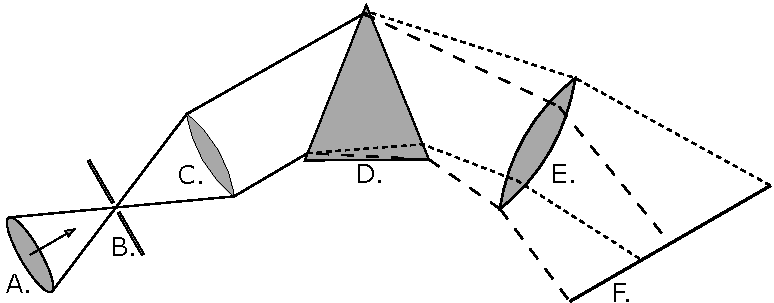
\includegraphics[width = 0.9\textwidth]{figures/2_spectrometer.pdf}
    \caption{Layout depicting the path light collected by a telescope would travel through a simple spectrometer.}
    \label{fig:spectrometer}
\end{figure}

% How it works
The simplest spectrometer schematic as shown in Figure \ref{fig:spectrometer} consists of incident light collected from the telescope's optics, labeled A, being focused onto a slit, labeled B, and passed through a collimator, labeled C. The collimator collimates the light allowing a dispersion element (such as a diffraction grating or prism), labeled D, to disperse the light into its constituent wavelengths. The resultant spectrum is focused by a focusing lens, labeled E, onto a focal plane, labeled F. Viewing optics are situated at the focal plane in the case of a spectroscope and a detector is situated at the focal plane in the case of a spectrograph.
\prgph

% Telescope optics
The telescope optics refers simply to all the components of a telescope necessary to acquire a focal point where the spectrometer, components labeled B - F, is situated. The focal point in most traditional telescope designs is fixed relative to the telescope and so the spectrometer may be mounted at that point. In cases where the telescope is designed to have a moving focal point relative to the telescope \cite[see][]{Arecibo, HET, SALT_design}, the spectrometer must also move along the telescope's focal path.
\prgph
\prgph

% SLIT
The slits function is to control the amount of incident light entering a spectrometer and, along with the exposure time of the detector, prevents over-exposures of bright sources on highly sensitive detectors \citep{TonkPracAmSpec}. If a source is spatially resolvable, or larger than the seeing conditions, the slit further acts to spatially limit the source to increase the spectral resolution, resulting in sharper features in the resultant spectrum.
\prgph

Without a slit the spectral resolution would be determined by the projected width of the source on the detector, or the seeing if the source was a star-like point source. Increasing the spectral resolution comes with the trade-off of decreasing the light collected from the source and thus acquiring a less intense resultant spectrum. Multiple spectra may be acquired simultaneously when the slit is positioned such that collinear sources lie along the slit.
%Spectroscopy done with no slit is commonly referred to as objective spectroscopy and, as the name suggests, the prism is situated just before the telescopes objective, the primary element of the telescope that focuses the collected light to the primary focus.
\prgph

% COLLIMATOR
The collimating lens functions to collimate the focused light from the telescope, ensuring that all light rays run parallel before reaching the dispersion element. Since the collimator accounts for the telescope's focus, the focal ratio of the collimator, $f_{1} / d_{1}$, should thus optimally match the focal ratio of the telescope, $f / D$, as seen in Equation \ref{eq:focal_ratio} to be most efficient and to not waste collecting area or material on too large a collimator.
% \prgph

\begin{equation}
    \frac{f}{D} = \frac{f_{1}}{d_{1}}
    \label{eq:focal_ratio}
\end{equation}

% From basic trigonometry and a small angle approximation, $\sin(\theta) \approx \theta$, Equation \ref{eq:small_angle} can be derived. From it, it can be seen that as the linear size, $D$, of most stellar objects is much smaller than the distance to those objects, $d$, and thus the incident light is already almost entirely collimated.

% \begin{equation}
% 	\theta (\arcsec) = 206265 \frac{D}{d}
% 	\label{eq:small_angle}
% \end{equation}

% DISPERSION ELEMENT
The dispersion element is the element that defines a spectrometer. As the name suggests, a dispersion element disperses the light incident on it into its constituent wavelengths and produces a spectrum. There are two types of dispersion elements, namely the prism and the diffraction grating, which operate on different principles, as discussed in Section \ref{subsec:dispersion}.
\prgph

% Focusing lens and FOCAL PLANE / Detector / Camera / CCD
% Can use \citep{CMOS_use} for CMOS use in general spectroscopy
%  - Spectroscopy and Spectrography
The focusing lens functions similarly to that of the telescope's optics but in this case focuses the dispersed light onto some receiver situated at the focal plane. As mentioned previously, an eye piece is fixed to the focal point for a spectroscope while a spectrograph employs a detector.
\prgph

The two most prevalent detector types in spectroscopy are the \gls{CCD} and \gls{CMOS} detectors. In astronomical spectroscopy however, sources are fainter and exposure times are much longer and so the \gls{CCD} detectors are by far the preferred detector as their output has a higher-quality and lower-noise when compared to \gls{CMOS} cameras under the same conditions \citep{CCDvsCMOS}.
\prgph

The \gls{CCD} is a detector composed of many thousands of pixels which can store a charge so long as a voltage is maintained across the pixels. Each pixel detects incoming photons using photo-sensitive capacitors through the photoelectric effect and converts the photons to a charge \citep{CCDastronomy}. There are also thermal agitation effects which introduce noise to the charge accumulated by a pixel, further discussed in Section \ref{subsec:calibration}. Once the exposure is finished the accumulated charge is read column by column, row by row, through an \gls{ADC}  which produces a two-dimensional array of `counts' with which information may be extracted from. Each \gls{CCD} image may be referred to by a name such as a bias, dark, flat field, or science image, which helps the observer differentiate the purpose of each image, also further discussed in Section \ref{subsec:calibration}.

\subsection{Dispersion Elements} \label{subsec:dispersion}
% https://spectroscopy.wordpress.com/2020/05/12/basics-on-prisms-and-diffraction-gratings-part-1/

Light can be broken up into its constituent wavelengths through two different physical phenomena, namely dispersion and diffraction, which dispersive elements use to create spectra. Dispersive prisms and diffractive gratings each have their strengths and weaknesses and a wide spectrum of instruments exist implementing both, or either, concepts. Regardless of the specific element, dispersive elements all have a resolving power, $R$, and an angular dispersion. Generally, while the angular dispersion is a more involved process to determine, the resolving power of a spectrograph can be measured as:
% \prgph

\begin{equation}
    R = \frac{\lambda}{FWHM}
    \label{eq:resolving_power}
\end{equation}

\noindent where $\lambda$ is the wavelength of an incident monochromatic beam and $FWHM$ refers to the width of the feature on the detector at half of its maximum intensity.
\prgph

%   - Prism
\begin{figure}[t]
    \centering
    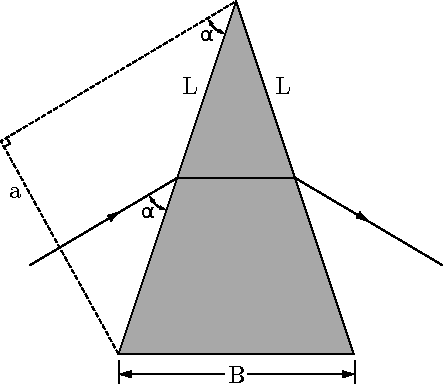
\includegraphics[width = 7cm]{figures/2_prism_diagram.pdf}
    \caption{Geometry of a prism refracting an incident monochromatic beam at a minimum deviation angle.}
    \label{fig:prism_diagram}
\end{figure}

The prism operates on the principle that the refractive index of light, $n$, varies as a function of its wavelength, $\lambda$. Prisms were the only dispersive elements available for early spectroscopic studies, but they were not without flaw.
% \prgph

\begin{equation}
    \frac{\partial \theta}{\partial \lambda} = \frac{B}{a}\frac{dn}{d\lambda}% \propto -\lambda^{-3}
    \label{eq:prism_angular_dispersion}
\end{equation}

The angular dispersion of a prism can be represented by Equation \ref{eq:prism_angular_dispersion} where the variables relate to Figure \ref{fig:prism_diagram} such that $\theta$ is the angle at which the refracted light differs from the incident light, $\lambda$ is the wavelength of the incident light, $B$ is the longest distance the beam would travel through the prism, and $a = L \sin(\alpha)$ is the cross-section of the incident beam where $L$ is the length of the transmissive surfaces and $\alpha$ is the incident angle of light to the prism surface. The refractive index of a material as a function of its wavelength, $n(\lambda)$, has several equations. Cauchy's equation, as given in Equation \ref{eq:Cauchy}, is a much simpler approximation of the refractive index that remains very accurate at visible wavelengths.
% \prgph

\begin{equation}
    n(\lambda) = A_{C} + \frac{B_{C}}{\lambda^{2}} + \frac{C_{C}}{\lambda^{4}} + \dots
    \label{eq:Cauchy}
\end{equation}

Equation \ref{eq:Cauchy}'s $A_{C}, B_{C}, C_{C}, \dots$ variables are called the Cauchy coefficients and have known values dependent on the material. Taking only the first term of the derivative of the Cauchy equation allows us to approximate the angular dispersion of a prism.

\begin{equation}
    \frac{\partial \theta}{\partial \lambda} = -\frac{B}{a}\frac{2B_{C}}{\lambda^{3}} \propto -\lambda^{-3}
    \label{eq:prism_angular_dispersion_approx}
\end{equation}

Equation \ref{eq:prism_angular_dispersion_approx} shows that the angular dispersion of a prism is wavelength dependent and furthermore that longer wavelengths are dispersed less than shorter wavelengths \citep{BirneyObsAstro, Hecht_optics}. The dependence of the angular dispersion, $d\theta/d\lambda$, on the wavelength, $\lambda$, is crucial for the formation of a spectrum but this cubic, non-linear, relation results in a non-linear spectrum. Since prisms rely on the refractive index of the material they are made of they have low angular dispersions.
\prgph

Multiple prisms can be used to increase the angular dispersion but as the dispersion is non-linear it becomes increasingly more difficult to calibrate. The more material and material boundaries the light must pass through the more its intensity decreases due to attenuation effects and Fresnel losses. Even so, the transmittance of modern prisms for their selected wavelength range is generally very high due to improved manufacturing methods as well as improved transmitting materials.
\prgph

%   - Diffraction grating
\begin{figure}[t]
    \centering
    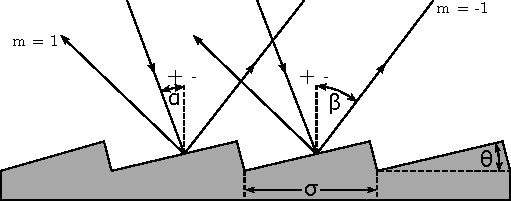
\includegraphics[width = 9cm]{figures/2_grating_diagram.pdf}
    \caption{Geometry of a reflective blazed grating refracting\\an incident monochromatic beam}
    \label{fig:grating_diagram}
\end{figure}

The diffraction grating operates on the principle that when light interacts with a grating where the groove size is comparable to the light's wavelength, the light is dispersed as a function of its wavelength through constructive and destructive interference. This interference results in multiple diffracted beams $m$, called orders, either side of a central reflected, or transmitted, beam such that $m \in Z$, where $m = 0$ is the non-dispersed, or reflected, beam.
% \prgph

\begin{equation}
    m\lambda = \sigma (\sin(\alpha) \pm \sin(\beta))
    \label{eq:grating_equation}
\end{equation}

% Link eq and fig
Equation \ref{eq:grating_equation} is referred to as the grating equation and its variables relate to Figure \ref{fig:grating_diagram} such that $m$ is the order of the diffracted beam being measured, $\lambda$ is the wavelength of the incident light, $\sigma$ is the groove spacing, $\alpha$ is the angle of incident light relative to the grating normal, and $\beta$ is the angle of diffraction relative to the grating normal. It is important to note that the sign of $\alpha$ and $\beta$ depend on whether the grating is reflective or transmissive. In the case of a reflective grating, such as in Figure \ref{fig:grating_diagram}, the signs of $\alpha$ and $\beta$ are the same relative to the grating normal, I.E. $\lambda = \sigma (\sin(\alpha) + \sin(\beta))$ for $m = 1$. In the case of a transmissive grating, the signs of $\alpha$ and $\beta$ are the opposite relative to the grating normal, I.E. $\lambda = \sigma (\sin(\alpha) - \sin(\beta))$ for $m = 1$.
\prgph

% Free Spectral range and Blazing
Equation \ref{eq:grating_equation} also describes how multiple wavelengths can share an angle of refraction when $m\lambda_{m} = (m + 1)\lambda_{m + 1}$. The regions of an order that do not overlap with another order are called the free spectral range. To account for the overlaps and increase the free spectral range an order-blocking filter may be used, and the diffraction grating may be blazed by an angle, $\theta$, such as in Figure \ref{fig:grating_diagram}. Blazing refers to the fact that the grooves on the surface of the grating are not symmetrical. The asymmetry of the grooves diffract the incident beam such that most of the incident beam's intensity is focused to a single order for a designated `blazed' wavelength, $\lambda_{b}$.
% \prgph

\begin{equation}
    m\lambda_{b} = 2\sigma\sin(\theta)\cos(\alpha - \theta)
    \label{eq:blaze_wavelength}
\end{equation}

\noindent where

\begin{equation}
    2\theta = \alpha + \beta
\end{equation}

% Angular dispersion
Taking the derivative of Equation \ref{eq:grating_equation} with respect to $\lambda$ and keeping $\alpha$ constant allows us to determine the angular dispersion of a diffraction grating.

\begin{equation}
    \frac{\partial \beta}{\partial \lambda} = \frac{m}{\sigma \cos(\beta)}
    \label{eq:grating_angular_dispersion}
\end{equation}

\noindent Substituting $m / \sigma$ with the grating equation gives

\begin{equation}
    \frac{\partial \beta}{\partial \lambda} = \frac{\sin(\alpha) + \sin(\beta)}{\lambda \cos(\beta)} \propto \lambda^{-1}
    \label{eq:grating_angular_dispersion_approx}
\end{equation}

Similarly to the dispersion of a prism, Equation \ref{eq:grating_angular_dispersion_approx} shows that the dispersion of a grating is wavelength dependent, but this dependence is only inversely proportional and thus more uniform across a wavelength range than that of a prism. Furthermore, shorter wavelengths are refracted less than longer wavelengths since there is no negative relation between the angular dispersion and the wavelength \citep{BirneyObsAstro, Hecht_optics}.
\prgph

% Grism and immersed grating
As mentioned before, multiple subgroups exist for both dispersive prisms and diffractive gratings. For prisms, along with the single and multiple prism setups mentioned above, there also exist grisms and immersed gratings. A grism (Grating Prism) refers to a transmissive grating etched onto one of the transmissive faces of a prism and allows a single camera to capture both spectroscopic and photometric images without needing to be moved, with and without the grism in the path of the beam of light, respectively. An immersed grating refers to a grism modified such that the transmissive grating is coated with reflective material. The primary source of dispersion for both grisms and immersive gratings is the grating and any aberration effects from the prism are negligible in comparison.
\prgph

\begin{figure}[t]
    \centering
    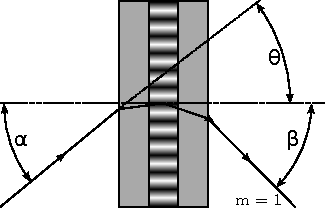
\includegraphics[width = 10cm]{figures/2_vph_grating.pdf}
    \caption{Geometry of a \gls{VPH} grating for an incident monochromatic beam of light.}
    \label{fig:vph_grating}
\end{figure}

% Echelle and VPH grating
% https://www.astro.ljmu.ac.uk/~ikb/vph.html
For gratings, along with transmissive and reflective gratings there also exist \gls{VPH} gratings. A \gls{VPH} grating consists of a photoresist, which is a light-sensitive material, sandwiched between two glass substrates. Diffraction is possible since the photoresist's refractive index varies near-sinusoidally perpendicularly to the gratings lines. This allows for sharper diffraction orders and low stray light scattering as compared to more traditional gratings but since blazing is not possible the efficiency is decreased. An echelle grating refers to two gratings set up such that the dispersed light from one is further diffracted by a second and allows for comparatively higher spectral resolutions when compared to more traditional grating setups. The gratings used as part of the echelle grating may be any type of dispersion element, but gratings are traditionally preferred due to the linearity of their resultant spectrum.
\prgph

\subsection{Detector and Spectroscopic Calibrations}\label{subsec:calibration}

Acquiring a spectrum from observations is more involved than simply reading out the data recorded on the \gls{CCD}. A raw science image, which is the raw counts of the observed source read from the \gls{CCD} with no calibrations applied, has on it a combination of useful science data as well as noise. The noise is a combination of random noise introduced through statistical processes and systematic noise introduced through the instrumentation and the observation conditions the source was observed under. This noise causes an uncertainty in the useful data and can be minimized, predominantly by calibrating for the systematic noise, but never fully removed \citep{CCDhandbook}.
\prgph

The dominant source of noise in a raw image is detector noise. \gls{CCD}'s are manufactured to have a small base charge in each pixel, called the `bias' current which allows the readout noise, a type of random noise, to better be sampled. There is also an unintentional additional charge which is linearly proportional to the exposure time and originates from thermal agitation of the \gls{CCD} material, called the `dark' current. The dark current can be minimized and possibly ignored if the \gls{CCD} is adequately cooled. These types of noise add to the charge held by a pixel and are thus considered additive.
\prgph

\begin{figure}[t]
    \centering
    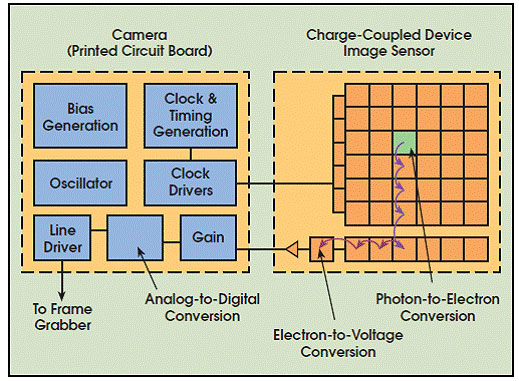
\includegraphics[width = 10cm]{figures/2_ccd.jpg}
    \caption{Diagram of a \gls{CCD}. Figure adapted from \citep{ccd_fig}}
    \label{fig:ccd_diagram}
\end{figure}


The \gls{CCD} is not a perfect detector and the efficiency of it and the optics of the telescope also contribute noise to the image. The efficiency of a \gls{CCD} is referred to as the Quantum Efficiency, and it is a measure of what percentage of light striking the detector is actually recorded and converted to a charge. The efficiency of the \gls{CCD} and telescope optics is also wavelength dependent and so the noise that results from them is more complex than that of additive noise. This type of noise is referred to as multiplicative noise.
\prgph

Each image taken by a \gls{CCD} will inherently have the additive types of noise in the image, and so bias and dark currents are the first types of noise to be accounted for by subtracting them from any subsequent images. Bias currents can be found by taking a bias image or by adding an overscan region to each image. A bias image is an image where the charges on the \gls{CCD} are reset and then immediately read off without exposing anything on the detector, effectively taking an image with zero exposure time. Alternatively, to save time during an observational run, overscan regions may be added to the images. An overscan region refers to adding a few cycles to the readout of each column of the \gls{CCD} such that the base current is read out and appended to each image.
\prgph

Dark currents can be found by taking an image with nothing exposed onto the detector for a certain exposure time. This resultant dark image can then be scaled to the science images exposure time since the dark current is linearly proportional to exposure time. When the detector is capable of being held at precise temperatures, dark images may be taken over multiple hours during the day to produce a high quality master dark image that may then be scaled and subtracted from all subsequent images.
\prgph

After the additive noise has been accounted for, the response from the pixels detecting the same incoming light are still not all the same due to the multiplicative noise which still needs to be accounted for. An image that has this noise accounted for is considered to be flat since all pixels share the same response to the incoming light. This noise can be measured by taking a `flat' image, or alternatively a flat-field, and multiple types of flats can be taken which all in essence image a uniformly illuminated region to determine the pixel-to-pixel response.
\prgph

Night sky flats are produced from science images where the images contain mostly sky. The science images are combined using the mode statistic which removes any celestial objects. This allows science images to be used for flat-fielding but at the cost of having a low \gls{SNR} because of the dim background sky. Dome flats are images taken of a flat surface inside the telescopes dome that has been uniformly and indirectly illuminated. These flats allow precise control of the light source and are also capable of being taken during the day. Finally, twilight flats are images taken of the twilight (or dawn) sky, when the Sun has just set, opposite the direction of the Sun at about $20\degr$ from zenith. Careful planning is required for twilight flats as the sky's brightness changes rapidly with the setting and rising of the Sun.
\prgph

A flat-field must be normalized before being used to correct any science images since it only acts to account for the pixel-to-pixel response and not for the additive errors. The normalized flat image, $F^{n}_{\lambda}(x,y)$ can be calculated as:

\begin{equation}
    F^{n}_{\lambda}(x,y) = \frac{F_{\lambda}(x,y) - B(x,y) - (\frac{t_{S}}{t_{D}})D(x,y)}{mode(F_{\lambda}(x,y) - B(x,y) - (\frac{t_{S}}{t_{D}})D(x,y))}
    \label{eq:norm_flat}
\end{equation}

\noindent where $F_{\lambda}(x,y)$ is the non-corrected flat image, $B(x,y)$ is the bias image, $D(x,y)$ is the dark image which is scaled by $t_{S}$ and $t_{D}$, the science image and dark image exposure times, respectively.
\prgph

The calibrated science image, $S^{*}_{\lambda}(x,y)$, which accounts for the bias and dark currents as well as the flat fielding can then be calculated as:

\begin{equation}
    S^{*}_{\lambda}(x,y) = \frac{S_{\lambda}(x,y) - B(x,y) - (\frac{t_{S}}{t_{D}})D(x,y)}{F^{n}_{\lambda}(x,y)}.
    \label{eq:science_cal}
\end{equation}

Multichannel \gls{CCD}'s are detectors that use either multiple \gls{CCD}'s or a \gls{CCD} with multiple output amplifiers which can be read out through multiple channels at the same time, increasing the detectors size while keeping the readout time constant. These \gls{CCD} setups need additional calibrations, specifically cross-talk corrections and mosaicking.
\prgph

Cross-talk noise refers to contamination that occurs during readout in one channel from another channel with a high signal and occurs because the signals can not be completely isolated from one another. Cross-talk corrections therefore account for this signal contamination between channels being read out at the same time \citep{CrossTalk}. Mosaicking is necessary for multichannel \gls{CCD}'s since the digitized signal read out from the detector has no reference of the physical location of the pixel it was detected at. Mosaicking therefore orients the data acquired from a multichannel detector correctly relatively to one another so that a single image is produced from the multiple channels read out from the detector.
\prgph

Finally, calibrations necessary for spectroscopy are limited to wavelength calibrations. Since the dispersion element breaks the incident light into its constituent wavelengths non-linearly, as discussed in Section \ref{subsec:dispersion}, the relation between the pixel on a detector and the wavelength of the light incident on it is unknown. Ideally, the spectrometer's optics would be modeled to produce a reliable pixel to wavelength calibration \citep[see E.g.][]{WavCalSpectraModel}, but this becomes increasingly more difficult for spectrometers with complex, non-sedentary, optical paths. Alternatively, a source with well-defined spectral features, with said features evenly populating the wavelength region of interest, such as in Figure \ref{fig:Ne_arc} may be observed. The observed frame is commonly referred to as an `arc' frame, after the arc lamps used to acquire the spectra, and should be observed alongside the science frames over the course of an observation run. It is important that the arc frame is observed at the same observing conditions and parameters as the science frames since the optical path will vary over the course of an observing run and for different observing parameters, invalidating previously acquired arc frames.
\prgph

\begin{figure}[t]
    \centering
    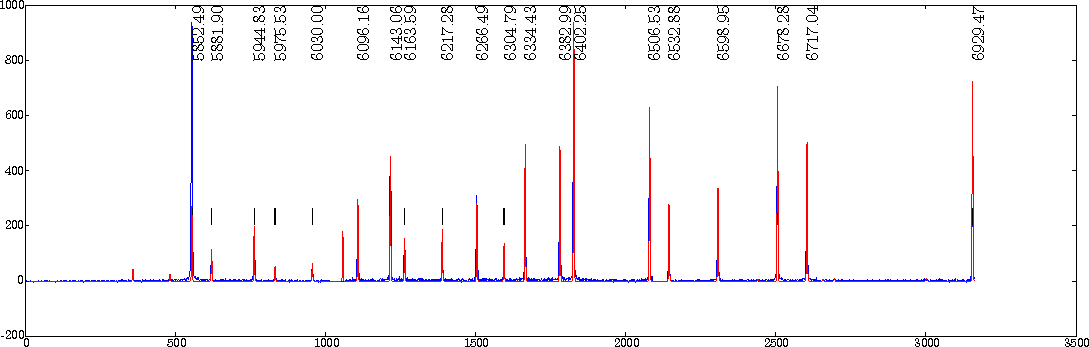
\includegraphics[width = 16cm]{figures/2_Ne_arc.pdf}
    \caption{Example of an arc spectrum for NeAr taken with \gls{SALT}'s \gls{RSS} using the PG1800 grating at a grating angle of $34.625$°, an articulation angle of $69.258$°, and covering a wavelength range of $\sim5600 - 6900$\angstrom. Plot adapted from \gls{SALT}'s published Longslit Line Atlases (as of 2023)\protect\footnotemark}
    \label{fig:Ne_arc}
\end{figure}
\footnotetext{\protect\href{http://pysalt.salt.ac.za/lineatlas/plot_line_neon.pdf}{NeAr plot} sourced from \protect\url{https://astronomers.salt.ac.za/data/salt-longslit-line-atlas/}}

The wavelength calibrations then consist of identifying a two-dimensional pixel to wavelength conversion function from the arc frame which may later be applied to calibrate the science frames. The two most common approximations for wavelength calibrations are the Chebyshev and Legendre polynomial approximations as found in Equations \ref{eq:chebyshev} and \ref{eq:legendre}, respectively. The Chebyshev polynomials are defined explicitly as:

\begin{equation}
    T_{n}(x) = \cos(n \cos^{-1}(x)),
    \label{eq:chebypolyexplicit}
\end{equation}

\noindent or recursively as:
\begin{equation}
    \begin{gathered}
        T_{0}(x) = 1 \\
        T_{1}(x) = x  \\
        T_{n}(x) = 2 x T_{n - 1}(x) - T_{n - 2}(x), \text{ for } n > 1
    \end{gathered}
    \label{eq:chebypoly}
\end{equation}

\noindent where $T$ is a Chebyshev polynomial\footnote{Denoted $T$ as a hold-over from the alternate spelling, `Tchebycheff'.} of degree $n$. Chebyshev polynomials are orthogonal when weighted by $1 / \sqrt{1 - x^{2}}$, meaning that the inner product of any two different polynomials, $T_{i}(x)$ and $T_{j}(x)$, over the range of $[-1, 1]$ is zero.

\begin{equation}
    \int_{-1}^{1} T_{i}(x) T_{j}(x) \frac{1}{\sqrt{1-x^{2}}} \,dx =
    \begin{cases}
        0,       & i \neq j     \\
        \pi / 2, & i = j \neq 0 \\
        \pi,     & i = j = 0
    \end{cases}
    \label{eq:chebyorth}
\end{equation}

A one or two-dimensional unknown calibration function may then be approximated by Chebyshev polynomials using:

\begin{equation}
    f(x) \approx \sum_{i = 0}^{N}  c_{i} T_{i}(u)
    \label{eq:chebyshev}
\end{equation}

\noindent or

\begin{equation}
    F(x, y) \approx \sum_{i = 0}^{N} \sum_{j = 0}^{M} c_{ij} T_{i}(u) T_{j}(v),
    \label{eq:chebyshev2D}
\end{equation}

\noindent respectively, where $N$ and $M$ are the desired $x$ and $y$ orders, $c_{ij}$ are the Chebyshev polynomial coefficients, and $u, v \in [-1, 1]$ are scaling factors to remap the variables $x, y \in [a, b]$ such that the orthogonality property of the Chebyshev polynomials holds true \citep{chebysurf, cheby2d}.

\begin{align}
    (u, v) & = \frac{2 (x, y) - a - b}{b - a} & (x, y) & = \frac{b - a}{2} (u, v) + \frac{a+b}{2}
    \label{eq:XtoUV}
\end{align}

% When the calibration function is known but the function cannot be evaluated, the coefficients, $c_{n}$, may be approximated by:

% \begin{equation}
%     c_{n} \approx \frac{2}{N} \sum_{k = 0}^{N - 1} f(x_{k}) T_{n}(x_{k})
%     \label{eq:chebycoeff}
% \end{equation}

% \noindent where:

% \noindent which returns the positions of the  x-intercepts.
% \prgph

The Chebyshev polynomials are more ideally suited for wavelength calibrations than standard polynomials since they are orthogonal and have minima and maxima located at $[-1, 1]$, as seen in Figure \ref{fig:chebyshev}. This means that the Chebyshev approximation is exact when $x = x_{n}$, where $x_{n}$ are the positions of the $n - 1$ x-intercepts of $T_{N}(x)$. This property greatly minimizes the error in the Chebyshev approximation, even at lower order approximations \citep{cheby}.

\begin{equation}
    x_{n} = \cos{\left(  \frac{\pi}{2} \frac{2 n + 1}{N} \right)}
\end{equation}

% \prgph

\begin{figure}[t]
    \centering
    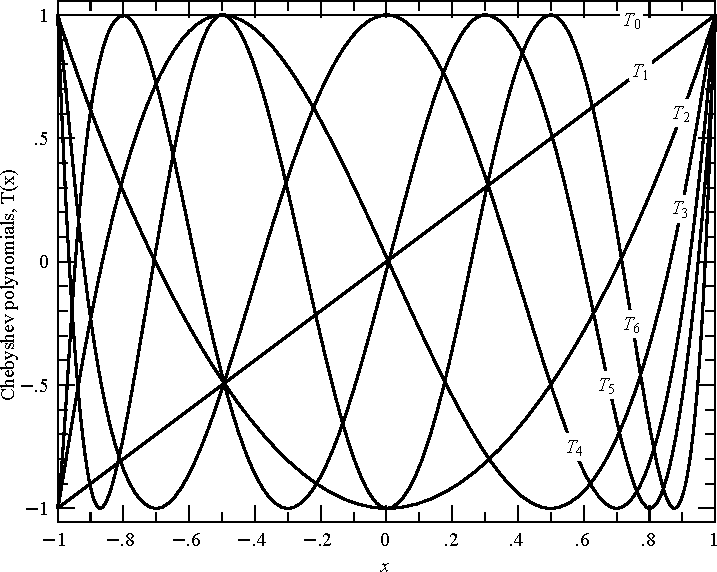
\includegraphics[width = 12cm]{figures/2_chebyshev.pdf}
    \caption{The first seven Chebyshev polynomials ($T_0$ through $T_{6}$) as defined by Equation \ref{eq:chebypoly} over the region $[-1, 1]$ for which they are orthogonal. Figure adapted from \citep{numerical_recipes} (2023)\protect\footnotemark}
    \label{fig:chebyshev}
\end{figure}
\footnotetext{Available digitally at \protect\href{http://numerical.recipes/book}{numerical.recipes}}

Similar to the Chebyshev polynomials, the Legendre polynomials may be defined explicitly as:

\begin{equation}
    P_{n}(x) = \frac{1}{2^{n} n!} \frac{d^{n}}{d x^{n}} (x^{2} - 1)^{n}
    \label{eq:legpolyexplicit}
\end{equation}

\noindent or recursively as:

\begin{equation}
    \begin{gathered}
        P_{0}(x) = 1 \\
        P_{1}(x) = x \\
        P_{n}(x) = \frac{2 n + 1}{n + 1} x P_{n - 1}(x) - \frac{n}{n + 1} P_{n - 2}(x), \text{ for } n > 1
    \end{gathered}
    \label{eq:legpoly}
\end{equation}

\noindent where P is a Legendre polynomial of degree n. Legendre polynomials are also orthogonal over the range $[-1, 1]$.
\prgph

\begin{equation}
    \int_{-1}^{1} P_{i}(x) P_{j}(x) \,dx =
    \begin{cases}
        0,                 & i \neq j \\
        \frac{2}{2 n + 1}, & i = j
    \end{cases}
    \label{eq:legorth}
\end{equation}

A one or two-dimensional unknown calibration function may then be approximated by Legendre polynomials using:

\begin{equation}
    f(x) \approx \sum_{n = 0}^{N} a_{n} P_{n}(u)
    \label{eq:legendre}
\end{equation}

\noindent or

\begin{equation}
    F(x, y) \approx \sum_{i = 0}^{N} \sum_{j = 0}^{M} a_{ij} P_{i}(u) P_{j}(v),
    \label{eq:Legendre2D}
\end{equation}

\begin{figure}[t]
    \centering
    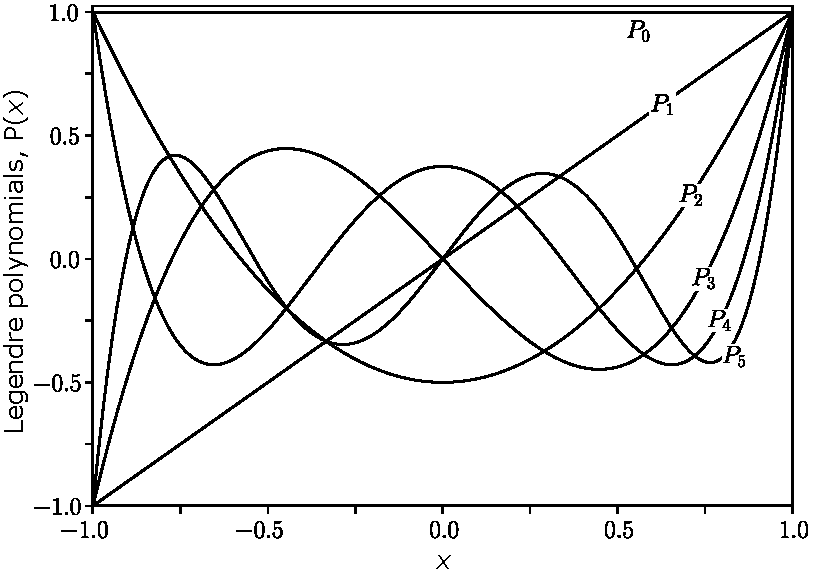
\includegraphics[width = 12cm]{figures/2_legendre.pdf}
    \caption{The first six Legendre polynomials ($P_0$ through $P_{5}$) as defined by Equation \ref{eq:legendre} over the region $[-1, 1]$ for which they are orthogonal. Figure adapted from Geek3, \protect\href{https://creativecommons.org/licenses/by-sa/3.0}{CC BY-SA 3.0}, via \protect\href{https://commons.wikimedia.org/wiki/File:Legendrepolynomials6.svg}{Wikimedia Commons} (2023)}
    \label{fig:legendre}
\end{figure}

\noindent respectively, where $N$ and $M$ are the desired $x$ and $y$ orders, $u$ and $v$ are the same mapping variable as in Equation \ref{eq:XtoUV}, and $a_{ij}$ are the Legendre polynomial coefficients. Legendre polynomials benefit from having the orthogonality condition with no weight necessary which makes their coefficients easier to compute but the error in a Legendre approximation of a function is greater than that of the error in a Chebyshev approximation for the same required order, $N$ (in one dimension) \citep{leg_cheb_relation}.
\prgph

Regardless of which set of polynomials is chosen, the polynomials are fit to the known (wavelength, pixel) pair using the least squares method. The resultant minimized function may then be used to convert the science frames from a (x pixel, y pixel) coordinate system to a (wavelength, y pixel) coordinate system.
\prgph


\section{Polarimetry}

% Origin of polarimetry (short history)
Both Huygens and Newton came to the conclusion that light demonstrates transversal properties \citep{Huygens, opticks}, which was later further investigated and coined as `polarization' by Malus \citep{Pol_Malus}. Malus also investigated the polarization effects of multiple materials including some of which were birefringent, such as optical calcite, which he referred to as Iceland spar after Bartholinus' investigations of the material \citep{Bartholinus}.

% Malus' law gives:
% \begin{equation}
%     I = I_{0} \cos^{2} \theta
%     \label{eq:Malus}
% \end{equation}
% \noindent where $I_{0}$ and $I$ are the Intensity of light before and after polarization, and $\theta$ is the orientation of the polarizer to the direction of propogation of the polarized light.
\prgph

Fresnel built on Malus' work showing that two beams of light, polarized at a right angle to one another, do not interfere, conclusively proving that light is transversal in nature, opposing the widely accepted longitudinal nature of light due to the prevalent belief in the ether. Fresnel later went on to correctly describe how polarized light is reflected and refracted at the surface of optical dielectric interfaces, without knowledge of the electromagnetic nature of light. Fresnel's equations for the reflectance and transmittance, $R$ and $T$, are defined as:

\begin{equation}
    \begin{gathered}
        R_{s} = \left\lvert \frac{Z_{2} \cos{\theta_{i}} - Z_{1} \cos{\theta_{t}}}{Z_{2} \cos{\theta_{i}} + Z_{1} \cos{\theta_{t}}} \right\rvert^{2} \\
        R_{p} = \left\lvert \frac{Z_{2} \cos{\theta_{t}} - Z_{1} \cos{\theta_{i}}}{Z_{2} \cos{\theta_{t}} + Z_{1} \cos{\theta_{i}}} \right\rvert^{2} \\
        T_{s} = 1 - R_{s} \\
        T_{p} = 1 - R_{p}
    \end{gathered}
    \label{eq:Fresnel}
\end{equation}

\noindent where $s$ and $p$ are the two polarized components of light perpendicular to one another, $Z_{1}$ and $Z_{2}$ are the impedance of the two media, and $\theta_{i}$, $\theta_{t}$, and $\theta_{r}$ are the angles of incidence, transmission, and reflection, respectively \citep{Fresnel}.
\prgph

Nicol was the first to create a polarizer, aptly named the Nicol prism, where the incident light is split into its two perpendicular polarization components, namely the ordinary and extraordinary beams. Faraday discovered the phenomenon where the polarization plane of light is rotated when under the influence of a magnetic field, known as the Faraday effect. Brewster calculated the angle of incidence, $\theta_{B}$, at which incident polarized light is perfectly transmitted through a transparent surface, with refractive indexes of $n_{1}$ and $n_{2}$, while non-polarized incident light is perfectly polarized when reflected and partially polarized when refracted.

\begin{equation}
    \theta_{B} = \arctan{\frac{n_{2}}{n_{1}}}
    \label{eq:Brewster}
\end{equation}

\begin{figure}[t]
    \centering
    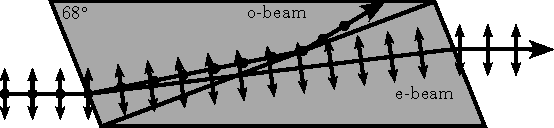
\includegraphics[width=10cm]{figures/2_Nicol_prism.pdf}
    \caption{Nicol prism diagram for incident non-polarized light.}
    \label{fig:Nicol_prism}
\end{figure}
\prgph

Stokes' work created the first consistent description of polarization and gave us the Stokes parameters which give an operational approach to polarization, discussed later in more detail \citep{Stokes}. Hale was the first to apply polarization to astronomical observations, using a Fresnel rhomb and Nicol prism as a quarter-wave plate and polarizer, respectively \citep{Hale_pre,Hale_post}. Wollaston also created a prism, similarly named the Wollaston prism, which allowed simultaneous observation of the ordinary and extraordinary beams due to the smaller deviation angle \citep{WollPrism}. Finally, Chandrasekhar's work furthered our understanding of astrophysical polarimetry by explaining the origin of polarization observed in starlight as well as mathematically modeling the polarization of rotating stars, which came to be named Chandrasekhar polarization \citep{chandrasekhar}.
\prgph

% how polarimetry works (most important) (in-depth)
% Polarimetry refers to the instrumental measurement of polarization.

% - theoretically
% Polarization ellipse from two perpendicular electric field vectors
% Maxwells electromagnetic light equations
% Stokes parameters
Maxwell's equations for an electromagnetic field propagating through a vacuum are given as:

\begin{equation}
    \begin{gathered}
        \nabla \cdot \matr{E} = 0 \\
        \nabla \cdot \matr{B} = 0 \\
        \nabla \times \matr{E} = - \frac{\partial \matr{B}}{\partial t} \\
        \nabla \times \matr{B} = \mu_{0} \epsilon_{0} \frac{\partial \matr{E}}{\partial t}
    \end{gathered}
    \label{eq:Maxwell}
\end{equation}

\noindent where $\matr{E}$ and $\matr{B}$ are the electric and magnetic field vectors, and $\mu_{0}$ and $\epsilon_{0}$ are the permeability and permittivity of free space, respectively, and related to the speed of light by $c~=~(\mu_{0} \epsilon_{0})^{-\frac{1}{2}}$. In a right-handed $(x, y, z)$ coordinate system, \hyperref[eq:Maxwell]{Maxwell's Equations} take a non-trivial solution for the electric field vector propagating along the $z$-axis, towards a hypothetical observer, of the form:

\begin{equation}
    \matr{E} = E_{x} \cos(\omega t - \Phi_{x}) \hat{\boldsymbol{x}} +
    E_{y} \cos(\omega t - \Phi_{y}) \hat{\boldsymbol{y}}
    \label{eq:Maxwell_sol}
\end{equation}

\noindent where $E_{x}$, $E_{y}$, $\Phi_{x}$, and $\Phi_{y}$ are all constants describing the amplitude and phase of the electric field vector in the $(x, y)$ plane. Rewriting Equation \ref{eq:Maxwell_sol} using complex values allows us to simplify the form of the solution to:

\begin{equation}
    \matr{E} = \Re(\matr{E}_{0} e^{-i \omega t})
    \label{eq:E_field_vector}
\end{equation}

\noindent where we only consider the real part of the equation, and where $\matr{E}_{0}$ is defined as:

\begin{equation}
    \matr{E}_{0} = E_{x} e^{i \Phi_{x}} \hat{\boldsymbol{x}} +
    E_{y} e^{i \Phi_{y}} \hat{\boldsymbol{y}}
    \label{eq:pol_vector}
\end{equation}

\noindent and is referred to as the polarization vector since it neatly contains the variables that are responsible for the polarization. Although the magnetic field is not discussed, it can be shown from \hyperref[eq:Maxwell]{Maxwell's Equations} that it is always defined as in phase and perpendicular to both the electric field vector and the direction of propagation with the form $\matr{B} = \Re(\matr{B}_{0} e^{-i \omega t})$.
\prgph

% Polarizing Ellipse
For an electric field vector with oscillations in some combination of the $x$ and $y$ axes, the tip of the vector sweeps out an ellipse. This ellipse is referred to as the polarization ellipse and has the form:

\begin{equation}
    \left( \frac{\matr{E}_{x}}{\matr{E}_{0, x}}\right)^{2} +
    \left( \frac{\matr{E}_{y}}{\matr{E}_{0, y}}\right)^{2} -
    \frac{2 \matr{E}_{x} \matr{E}_{y}}{\matr{E}_{0, x} \matr{E}_{0, y}} \cos\Phi =
    \sin^{2} \Phi
    \label{eq:pol_ellipse}
\end{equation}

\noindent where $\Phi = \Phi_{x} - \Phi_{y}$ is the phase difference. The degree of polarization for the polarization ellipse is related to the eccentricity of the ellipse and the angle at which it is rotated relates to the polarization angle. Because $\matr{E}_{0, x}$, $\matr{E}_{0, y}$, $\Phi_{x}$, and $\Phi_{y}$ are constant, the resultant polarization ellipse is fixed as the wave continues to propagate. We may then manipulate Equation~\ref{eq:pol_ellipse} to produce the polarization parameters:

\begin{figure}[t]
    \centering
    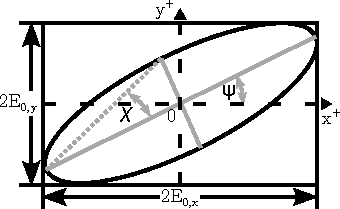
\includegraphics[width=6cm]{figures/2_pol_ellipse.pdf}
    \caption{The polarization ellipse for an electric field vector propagating through free space.}
    \label{fig:pol_ellipse}
\end{figure}


\begin{gather*}
    (E_{x}^{2} + E_{y}^{2})^{2} - (E_{x}^{2} - E_{y}^{2})^{2} - (2 E_{x} E_{y} \cos \Phi)^{2} = (2 E_{x} E_{y} \sin \Phi)^{2} \\
    \therefore P_{I}^{2} - P_{Q}^{2} - P_{U}^{2} = P_{V}^{2} \\
    \therefore P_{I}^{2} = P_{Q}^{2} + P_{U}^{2} + P_{V}^{2}
\end{gather*}

\noindent where

\begin{equation}
    \begin{gathered}
        P_{I} = E_{x}^{2} + E_{y}^{2} \\
        P_{Q} = E_{x}^{2} - E_{y}^{2} \\
        P_{U} = 2 E_{x} E_{y} \cos \Phi \\
        P_{V} = 2 E_{x} E_{y} \sin \Phi
    \end{gathered}
    \label{eq:pol_params}
\end{equation}
\prgph

There is, however, a seemingly small albeit major shortcoming of the polarization as defined in Equation~\ref{eq:pol_params}, the polarization ellipse as represented by Figure~\ref{fig:pol_ellipse} deals only with a single transverse wave and is incapable of handling a wave-packet made up of multiple waves. This is because the waves making up a wave-packet will not share their polarization properties and will temporally vary from one another. By taking the time average of the waves in a wave-packet this temporal variation may be eliminated.

\begin{equation}
    \avg{\matr{E}_{i} \matr{E}_{j}} = \lim_{T \rightarrow \infty} \frac{1}{T} \int_{0}^{T} \matr{E}_{i} \matr{E}_{j}\,dt, \text{ for } i, j \in (x, y)
\end{equation}

\noindent where $T$ is the total averaging time over electric field vectors $\matr{E}_{i}$ and $\matr{E}_{j}$. Equation~\ref{eq:pol_params} now simplifies to:

\begin{equation}
    \matr{S} =
    \begin{pmatrix}
        S_{0} \\
        S_{1} \\
        S_{2} \\
        S_{3}
    \end{pmatrix}
    =
    \begin{pmatrix}
        I \\
        Q \\
        U \\
        V
    \end{pmatrix}
    =
    \begin{pmatrix}
        \avg{E_{x}^{2}} + \avg{E_{y}^{2}} \\
        \avg{E_{x}^{2}} - \avg{E_{y}^{2}} \\
        \avg{2 E_{x} E_{y} \cos \Phi}     \\
        \avg{2 E_{x} E_{y} \sin \Phi}
    \end{pmatrix}
    \label{eq:Stokes_params}
\end{equation}

\noindent where $S_{0}$ -- $ S_{3}$ are referred to as the Stokes (polarization) parameters. This time averaging is what previous definitions of polarization failed to account for and as such they were only able to account for beams of completely polarized light. For a reference direction which defines the direction of the $x$-axis of our coordinate system, the Stokes parameters are physically described as follows: the $Q$ Stokes parameter is defined as the difference between the amount of photons oscillating parallel and perpendicular to the reference direction, the $U$ Stokes parameter is defined as the difference between the amount of photons oscillating at $45\degr$ and $135\degr$ counter-clockwise from the reference direction, and the $V$ Stokes parameter is defined as the difference between the amount of photons with right-handed (positive, clockwise) circular polarization and left-handed (negative, counter-clockwise) circular polarization \citep{Stokes}.
\prgph

Using the \hyperref[eq:Stokes_params]{Stokes parameters}, we can now account for partially polarized light such that:

\begin{equation}
    I^{2} \geq  Q^{2} + U^{2} + V^{2},
\end{equation}

\noindent where it should be noted that $(I, Q, U, V)$ represent the partial polarization parameters and are related to $(P_{I}, P_{Q}, P_{U}, P_{V})$ since the polarization may be partial. In general, and henceforth, $(P_{I}, P_{Q}, P_{U}, P_{V})$ are relative quantities normalized to the intensity, where

\begin{align}
    P_{I} & = 1, & P_{Q} & = \frac{Q}{I}, & P_{U} & = \frac{U}{I}, \text{   and } & P_{V} & = \frac{V}{I}.
    \label{eq:norm_Stokes}
\end{align}
% \prgph

Similar to the polarization ellipse, the Stokes parameters may be represented pictorially using the Poincar{\'e} sphere in spherical coordinates $(IP, 2 \Psi, 2 \chi)$, where $I$ denotes the total intensity and $P$ the degree of polarization, or the ratio of polarized to non-polarized light in the wave-packet, $\Psi$ denotes the polarization angle. It should be noted that the Poincar{\'e} sphere also uses the normalized Stokes parameters $(S_{0} = 1)$ as defined above in equation~\ref{eq:norm_Stokes}.

\begin{equation}
    \begin{gathered}
        I = S_{0} \\
        P = \frac{\sqrt{S_{1}^2 + S_{2}^2 + S_{3}^2}}{S_{0}}, \text{ for } 0 \leq P \leq 1 \\
        2 \Psi = \arctan \frac{S_{2}}{S_{1}} \\
        2 \chi = \arctan \frac{S_{3}}{\sqrt{S_{1}^{2} + S_{2}^{2}}}
    \end{gathered}
    \label{eq:poincare_coords}
\end{equation}

\begin{figure}[t]
    \centering
    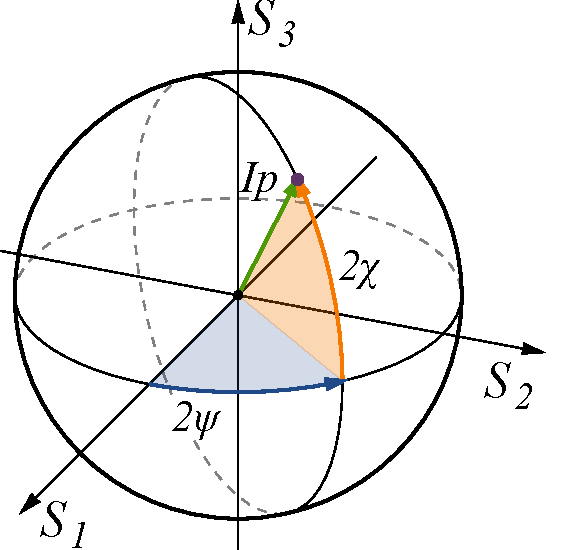
\includegraphics[width=6cm]{figures/2_poincare_sphere.pdf}
    \caption{The Poincar{\'e} sphere describing the polarization properties of a wave-packet propagating through free space. Figure adapted from \protect\href{https://commons.wikimedia.org/wiki/File:Poincaré_sphere.svg}{Wikimedia Commons} (2023)}
    \label{fig:poincare}
\end{figure}
\prgph

% The now time-invariant \hyperref[fig:pol_ellipse]{polarization ellipse} may now be defined in terms of the Stokes parameters as:

% Special cases, (1, \pm1, 0, 0), (1, 0, \pm1), (1, 0, 0, \pm1), (1, 0, 0, 0)
% Mueller matrix
% \citep{pol_in_spectra}

\begin{figure}[t]
    \centering
    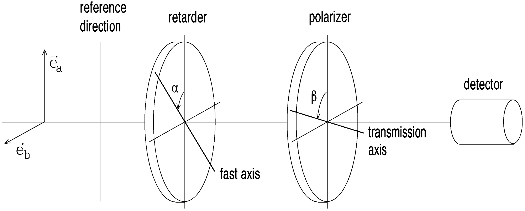
\includegraphics[width=1\textwidth]{figures/2_polarimeter.pdf}
    \caption{Diagram of an ideal polarimeter. Figure adapted from \cite{pol_in_spectra}.}
    \label{fig:polarimeter}
\end{figure}

% - practically
% Waveplate and polarizer
Except for polarimetry in the radio-wavelength regime, the polarization of a beam can not be directly measured. The polarization properties may, however, be recovered from the beam through manipulation of the four constants mentioned in Equation~\ref{eq:Maxwell_sol}. This so-called manipulation is achieved by passing the beam through optical elements which vary the beam for differing amplitudes and phases. These matrix operations may be represented by their corresponding Mueller matrices. For ideal components, the resultant beam $\matr{S}^{\prime}$ after passing through an optical element is given by

\begin{equation}
    \matr{S}^{\prime} = \matr{M} \matr{S}
\end{equation}

\noindent where $\matr{S}$ is the beam incident on the optical element and $\matr{M}$ represents the $4 \times 4$ Mueller matrix representing the optical element. Mueller matrices are especially useful when dealing with paths through optical elements as they observe the `train' property \citep{Mueller_train}. This means that an incoming beam $\matr{S}$ passing, in order, through elements with known Mueller matrices $(\matr{M}_{0}, \dots, \matr{M}_{N})$ results in an outgoing beam $\matr{S}^{\prime}$ such that:

\begin{equation}
    \matr{S}^{\prime} = \matr{M}_{N} \dots \matr{M}_{0} \matr{S}
    \label{eq:mueller_train}
\end{equation}
% \prgph

Some Mueller Matrices are given below with angles related to those in Figure~\ref{fig:polarimeter}, measured counter-clockwise in a right-handed coordinate system.

\paragraph*{General rotation}
The Mueller matrix for coordinate space rotations about the origin by an angle $\theta$.
\begin{equation}
    \matr{R}(\theta) =
    \begin{bmatrix}
        1 & 0              & 0             & 0 \\
        0 & \cos 2 \theta  & \sin 2 \theta & 0 \\
        0 & -\sin 2 \theta & \cos 2 \theta & 0 \\
        0 & 0              & 0             & 1 \\
    \end{bmatrix}
    \label{matrix:rotate}
\end{equation}

\paragraph*{General linear retardance}
The Mueller matrix for retardance where $\alpha$ is the angle between the incoming vector and fast axis, and $\delta$ is the retardance introduced by the retarder. The retarder is often referred to by this retardance, e.g. if the retardance is $\delta = \pi$ or $\pi / 2$ $radians$, the retarder is referred to as a half- or quarter-wave plate, respectively.
\begin{equation}
    \matr{W}(\alpha, \delta) =
    \begin{bmatrix}
        1 & 0                                                 & 0                                                 & 0                          \\
        0 & \cos^{2} 2 \alpha + \sin^{2} 2 \alpha \cos \delta & \cos 2 \alpha \sin 2 \alpha  (1 - \cos \delta)    & \sin 2 \alpha \sin \delta  \\
        0 & \cos 2 \alpha \sin 2 \alpha  (1 - \cos \delta)    & \cos^{2} 2 \alpha \cos \delta + \sin^{2} 2 \alpha & -\cos 2 \alpha \sin \delta \\
        0 & -\sin 2 \alpha \sin \delta                        & \cos 2 \alpha \sin \delta                         & \cos \delta                \\
    \end{bmatrix}
    \label{matrix:retarder}
\end{equation}

\paragraph*{General linear polarization}
The Mueller matrix for linear polarization where $\beta$ is the angle between the incoming vector and transmission axis.
\begin{equation}
    \matr{P}(\beta) = \frac{1}{2}
    \begin{bmatrix}
        1            & \cos 2 \beta              & \sin 2 \beta              & 0 \\
        \cos 2 \beta & \cos^{2} 2 \beta          & \cos 2 \beta \sin 2 \beta & 0 \\
        \sin 2 \beta & \sin 2 \beta \cos 2 \beta & \sin^{2} 2 \beta          & 0 \\
        0            & 0                         & 0                         & 0 \\
    \end{bmatrix}
    \label{matrix:polarizer}
\end{equation}
\prgph

These matrices in combination with the chain rule in Equation~\ref{eq:mueller_train} allow us to describe how the Stokes parameters would change when passing through various optical elements. For a setup similar to Figure~\ref{fig:polarimeter}, we can vary the retandance angle, $\alpha$, and polarization angle, $\beta$, for a wave plate with a relative phase difference, $\gamma$, to acquire a system of equations that we can solve to retrieve the Stokes polarization parameters \citep{waveplate_in_specpol}.

\begin{equation}
    \begin{split}
        S(\alpha, \beta, \gamma) \propto \frac{1}{2} \{ I & + [Q \cos2\alpha + U \sin2\alpha] \cos(2\beta - 2\alpha) \\
        & - [Q \sin2\alpha + U \cos2\alpha] \sin(2\beta - 2\alpha) \cos\gamma \label{eq:Stokes_intensity} \\
        & + V \sin(2\beta - 2\alpha)\sin\gamma \}
    \end{split}
\end{equation}
% \prgph

Several or more frames taken under differing configurations may be used to reduce the system of equations, but it is possible to extract the Stokes polarization parameters using only four frames for well-chosen configurations. The first three configurations do not use the waveplate, i.e. $\alpha = 0\degr$, but use polarizer angles of $\beta \in {0\degr, 45\degr, 90\degr}$, and the last configuration (to determine $S_{3}$ or $V$) uses a retardance of $\alpha = 90\degr$ and a polarizer angle of $\beta = 45\degr$.
\prgph

From Equation~\ref{eq:Stokes_intensity} we see that the polarizing element is the driving element of a polarizer as the first three Stokes parameters ($S_{0-2}$, or $I$, $Q$, and $U$) can be found by changing only the polarizing elements angle, $\beta$.
% \prgph

\paragraph{Wave plates}
Wave plates, also commonly referred to as retarders, are generally made from optically transparent birefringent crystals. A wave plate has a fast and slow axis, which are perpendicular to one another and both perpendicular to an incident beam. Due to the birefringence of the wave plate medium, the phase velocity of the beam polarized parallel to the fast axis, namely the extraordinary beam, slightly increases while that of the beam polarized parallel to the slow axis, namely the ordinary beam, remains unaffected \citep{Hecht_optics}.
\prgph

This introduces a relative phase difference between the two beams, $\gamma$, which is given by

\begin{equation}
    \gamma = \frac{2 \pi \Delta n L}{\lambda_{0}}
\end{equation}

\noindent where $\Delta n$ and $L$ refer to the birefringence and thickness of the wave plate medium, respectively, and $\lambda_{0}$ refers to the vacuum wavelength of the beam.
\prgph

This relative phase difference determines the name of the wave plate, such as the half- and quarter-wave plates referring to the $\gamma = m(\pi/2) $ and $\gamma = m(\pi/4)$ for $m \in Z^{+}$, respectively, which are also the most commonly used wave plates. Phase differences with an integer multiple of one another still relate to the same phase difference and are referred to as multiple-order wave plates. Multiple multiple-order wave plates can be combined by alternatively aligning the fast axis of one to the slow axis of another to create a compound zero-order wave plate. When the phase difference of the wave plate is not an integer difference it is referred to as a zero-order wave plate \citep{Hale_birefringence}.
% \prgph

\paragraph{Polarizers}
Polarizers are typically made from two prisms, of a birefringent material, cemented together with an optically transparent adhesive. The actual effect of separating the perpendicular polarization components is achieved using varying effects, namely through:
\begin{itemize}
    \item absorption of one of the polarized components, such as in Polaroid polarizing filters,
    \item total internal reflection of a single polarized component, such as in a Nicol prism (Figure~\ref{fig:Nicol_prism}),
    \item Refraction of a single polarized component, such as in a Rochon prism (Figure\ref{fig:Rochon_prism}), or
    \item Refraction of both polarization components in differing directions, such as in a Wollaston prism (Figure~\ref{fig:Wollaston_prism}).
\end{itemize}
% \prgph

\begin{figure}[t]
    \centering
    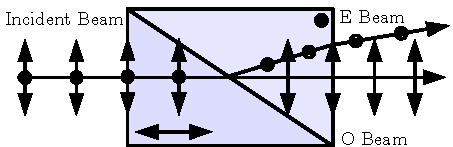
\includegraphics[width=0.5\textwidth]{figures/2_rochon.pdf}
    \caption{Diagram of a Rochon prism. Figure adapted from \protect\href{https://commons.wikimedia.org/wiki/File:Rochon_Prism.svg}{Wikimedia Commons} (2023)}
    \label{fig:Rochon_prism}
\end{figure}

\begin{figure}[t]
    \centering
    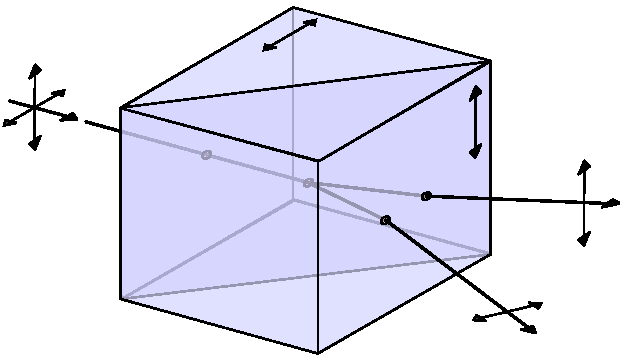
\includegraphics[width=0.5\textwidth]{figures/2_wollaston.pdf}
    \caption{Diagram of a Wollaston prism. Figure adapted from \protect\href{https://commons.wikimedia.org/wiki/File:Wollaston-prism.svg}{Wikimedia Commons} (2023)}
    \label{fig:Wollaston_prism}
\end{figure}

\paragraph{Wollaston prisms}
The Wollaston prism consists of two prisms consisting of a birefringent monoaxial material, cemented together with an optically transparent adhesive along their hypotenuses with their optical axes orthogonal, as seen in Figure~\ref{fig:Wollaston_prism}. The Wollaston prism is a common optical polarizing element in astrophysical polarimetry which separates an incident beam into two linearly polarized beams, orthogonal to one another, as expected of a polarizer, but which returns the two beams deviated from their common axis equally. The deviation angle is determined by the right-angle prism base angles \citep{wollaston}.
\prgph

A Wollaston prisms benefit over simpler elements, as listed previously, is that a single frame allows for the observation of a set of orthogonal polarization configurations. This halves the observational time required to collect enough data to calculate the Stokes parameters, at the cost of an increase in calibration and reduction difficulty.
% \prgph

\subsection{Polarimetric calibrations}\label{subsec:pol_cal}

% Corrections Related to the Detector
Similar to Section~\ref{subsec:calibration}, polarimetric calibrations are necessary when dealing with a polarimeter, though as the optical elements differ the calibrations similarly differ. Corrections and calibrations related to the \gls{CCD} remain unchanged while those related to correcting for the optical elements only need to be modified to correct for polarization instead of wavelength.
\prgph

% Flat-fielding, Extraction of the O and E Ray Images
% The most notable feature of an exposure taken by a polarimeter, specifically a polarimeter which produces both the $O$- and $E$-beams simultaneously, is the presence of two images of the same area of sky with the target source along with any additional sources present in both images.
Once the \gls{CCD} calibrations have been completed, the polarization intrinsic to the optical elements needs to be accounted for such that the pixel-to-pixel response is uniform. Flat-fielding can once again be used to correct for this. The flats taken for polarimetry, however, introduce an additional challenge as the targets for conventional flats are polarized, such as twilight and dome flats which are polarized by light scattering in the atmosphere and the reflective surface of the dome, respectively.
\prgph

If no unpolarized flat images can be taken for flat field calibrations then, when possible due to the polarimeter design, the wave plate may be constantly rotated to act as a depolarizing element and is effective so long as the wave plate rotates faster than the flat exposure time. Alternatively, spatially constant polarized flats may be used with the added restriction that science and flat images have more than the minimum two images taken. These frames may be redundant since the $O$- and $E$-beams differ by $\pi / 4$ but this introduced redundancy allows for the cancellation of any uniform polarization. More redundant pairs observed (up to the maximum redundancy of $16$) allow for a more efficient cancellation of the uniform polarization but cost exposure time as well as a flat image which is time-independent. In any case, when the flat contains any polarization, the removal of the uniform polarization  from the science frames is left for when the polarization is calculated \citep{polarimetry_error}.
\prgph

After calibrations for the \gls{CCD} and light path are accounted for, the $O$- and $E$-beams can be extracted and further reduced. The extraction depends heavily on the layout of the polarimeter but often a simple cropping of the differing sections is enough to separate the two images.
\prgph

% Image Alignment
The matching dual images need to be aligned once they have been extracted such that the sources present in them overlap. The Wollaston prism needs to be corrected for as it introduces a Wollaston prism beam deviation. The alignment is crucial as the comparison of the dual images is what allows astronomers to calculate the polarization properties.
\prgph

% Sky Subtraction
The polarization introduced by the sky needs to be removed as it will influence the polarization results of the target source. Thankfully, the background polarization is an additive type of noise and may be subtracted out across the frames. This subtraction should be done for each image in the frame, however, as the background intensity of each image will differ as the background polarization differs.


\section{Spectropolarimetry} % In depth

As the name suggests, spectropolarimetry is the measurement of the polarization of light for a chosen spectral range and provides results of not only spectra but also polarization parameters across the spectral range. The history of spectropolarimetry is one limited by the constituent elements of spectropolarimeters, namely spectrometers and polarimeters. The most notable historical contributions unrelated to spectroscopy or polarimetry are those of spectropolarimetric studies instead of instrumental developments.
\prgph

\todo{Figure of spectropolarimeter, reference}
\begin{figure}[t]
    \centering
    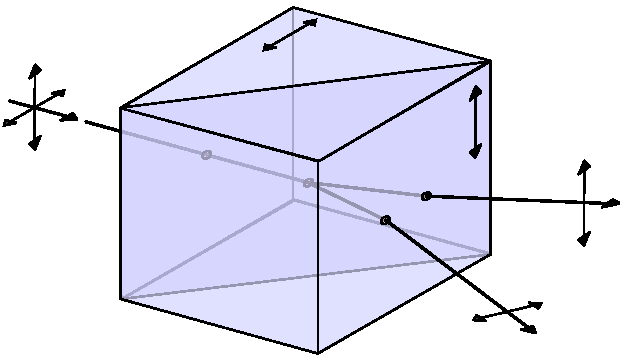
\includegraphics[width=0.5\textwidth]{figures/2_wollaston.pdf}
    \caption{Diagram of an ideal spectropolarimeter. Figure adapted from \protect\href{https://commons.wikimedia.org/wiki/File:Wollaston-prism.svg}{Wikimedia Commons} (2023)}
    \label{fig:spectropolarimeter}
\end{figure}

Along with common points of consideration when developing any instrumentation for observational astronomy, such as resolution and sensitivity, spectropolarimeters need to consider both the spectral range and any inherent polarization that may be introduced by the any elements within the light path.
\prgph

Time is another constraint for spectropolarimetry as, depending on the target of observation, the incident light is split up by wavelength as well as by polarization states. This `double' dividing of the incident light results in increased exposure times of not only target frames but also (time-dependent) calibration frames when compared to more traditional photometric observations.

\todo{
    \begin{itemize}
        \item How spectropolarimetry works in-depth (both practically and theoretically, I.E. frames, traces, O and E beams, etc.).
        \item Uses and what its use in astrophysics is.
    \end{itemize}
}

\subsection{Spectropolarimetric calibrations}

\todo{Figure of spectropolarimetric exposure, and caption}
\begin{figure}[t]
    \centering
    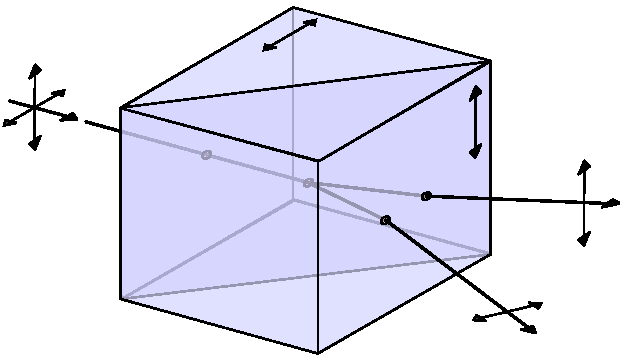
\includegraphics[width=0.5\textwidth]{figures/2_wollaston.pdf}
    \caption{A spectropolarimetric target exposure of \dots.}
    \label{fig:specpol_exposure}
\end{figure}

Spectropolarimetric calibrations are more involved when compared to the previous calibration discussions (Sections~\ref{subsec:calibration},~\ref{subsec:pol_cal}). More exposures are required to acquire enough redundancy for the calculation of all Stokes parameters, and the combination of calibrations discussed previously accounting for wavelength as well as polarization must both be implemented.
\prgph

\todo{Wavelength calibrations most important for spectroscopy just as frame alignment most important for polarimetry, both important for spectropolarimetry.}

\section{The South African Large Telescope} % Basics, not in depth

\gls{SALT} is a 10 m class optical/near-infrared telescope situated at the \gls{SAAO} field station near Sutherland, South Africa \citep{SALT_optical_design}. The operational design was based off of the \gls{HET} situated at McDonald Observatory, Texas, which limits the pointing of the telescope's primary mirror to a fixed elevation (37$\degree$ from zenith in the case of SALT) while still allowing for full azimuthal rotation \citep{HET}. Both SALT and HET utilize a spherical primary mirror which is stationary during observations and a tracker housing most of the instrumentation that tracks the primary mirrors spherically shaped focal path. Figure \ref{fig:SALT_telescope} depicts \gls{SALT}'s tracker (top left), supporting structure, and primary mirror (bottom right).

\begin{figure}[t]
    \centering
    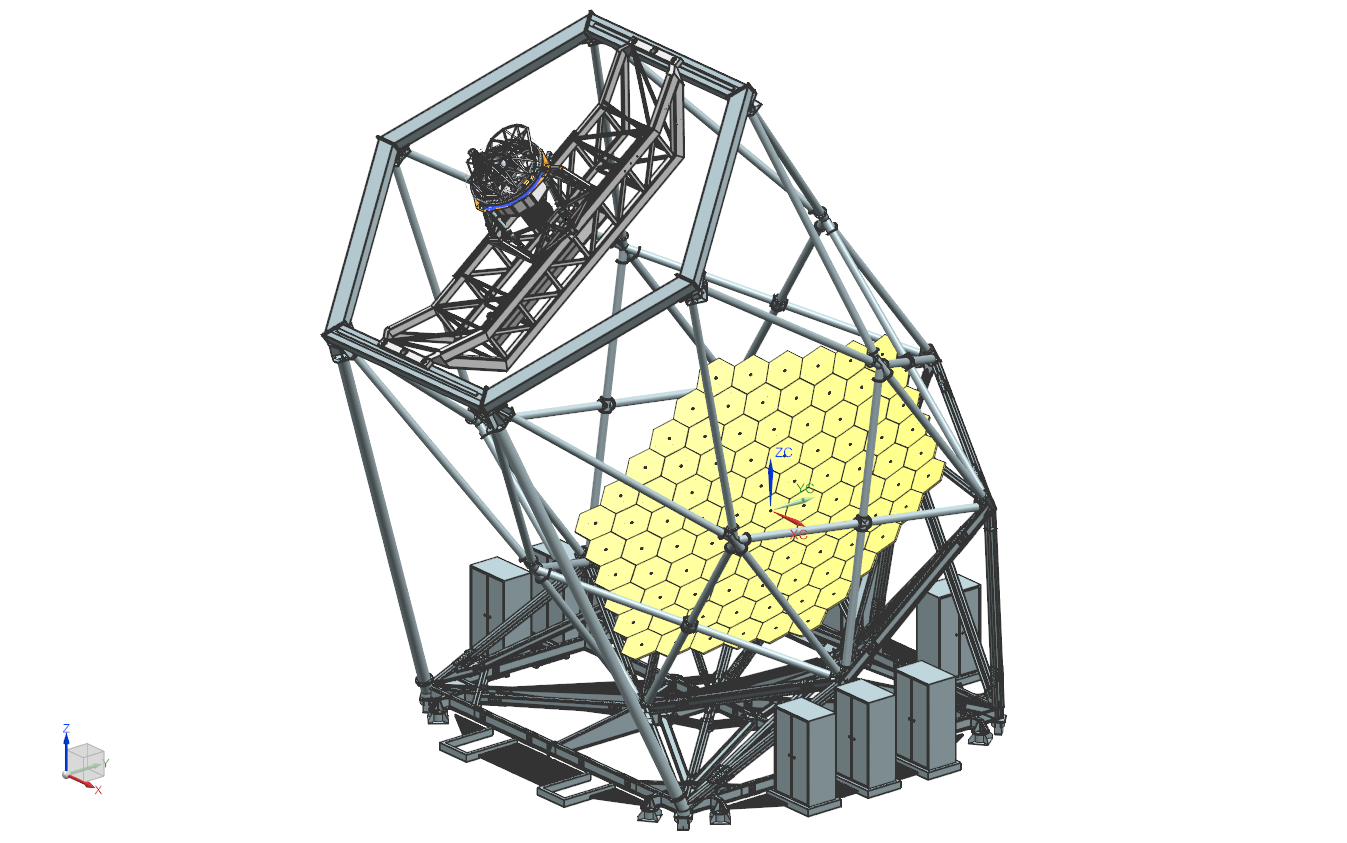
\includegraphics[width = 15cm]{figures/2_SALT_telescope.png}
    \caption{The tracker, supporting structure, and primary mirror of SALT. Figure adapted from the SALT call for proposals (2022)\protect\footnotemark}
    \label{fig:SALT_telescope}
\end{figure}
\footnotetext{\protect\url{http://pysalt.salt.ac.za/proposal_calls/current/ProposalCall.html}}

\subsection{The primary mirror}

The primary mirror is composed of 91 individual 1 m hexagonal mirrors which together form an 11 m segmented spherical mirror. Each mirror segment can be adjusted by actuators allowing the individual mirrors to approximate a single monolithic spherical mirror. The fixed elevation means that SALT's primary mirror has a fixed gravity vector allowing for a lighter, cost-effective supporting structure when compared to that of a more traditional altitude-azimuthal mount but with the trade-off that the control mechanism and tracking has increased complexity \citep{SALT_design}.

\subsection{Tracker and tracking}

During observations the primary mirror is stationary and the tracker tracks celestial objects across the sky by moving along the primary focus. The tracker is capable of 6 degrees of freedom with an accuracy of ~5 $\mu$m and is capable of tracking $\pm$6$\degree$ from the optimal central track position. Targets at declinations from 10.5$\degree$ to -75.3$\degree$, as shown in Figure \ref{fig:SALT_visibility} are accessible during windows of opportunity. As the tracker moves along the track the effective collecting area varies and thus SALT has a varying effective diameter of $\sim7$ m to 9 m when the tracker is furthest and closest to the optimal central position, respectively.
\prgph

\begin{figure}[t]
    \centering
    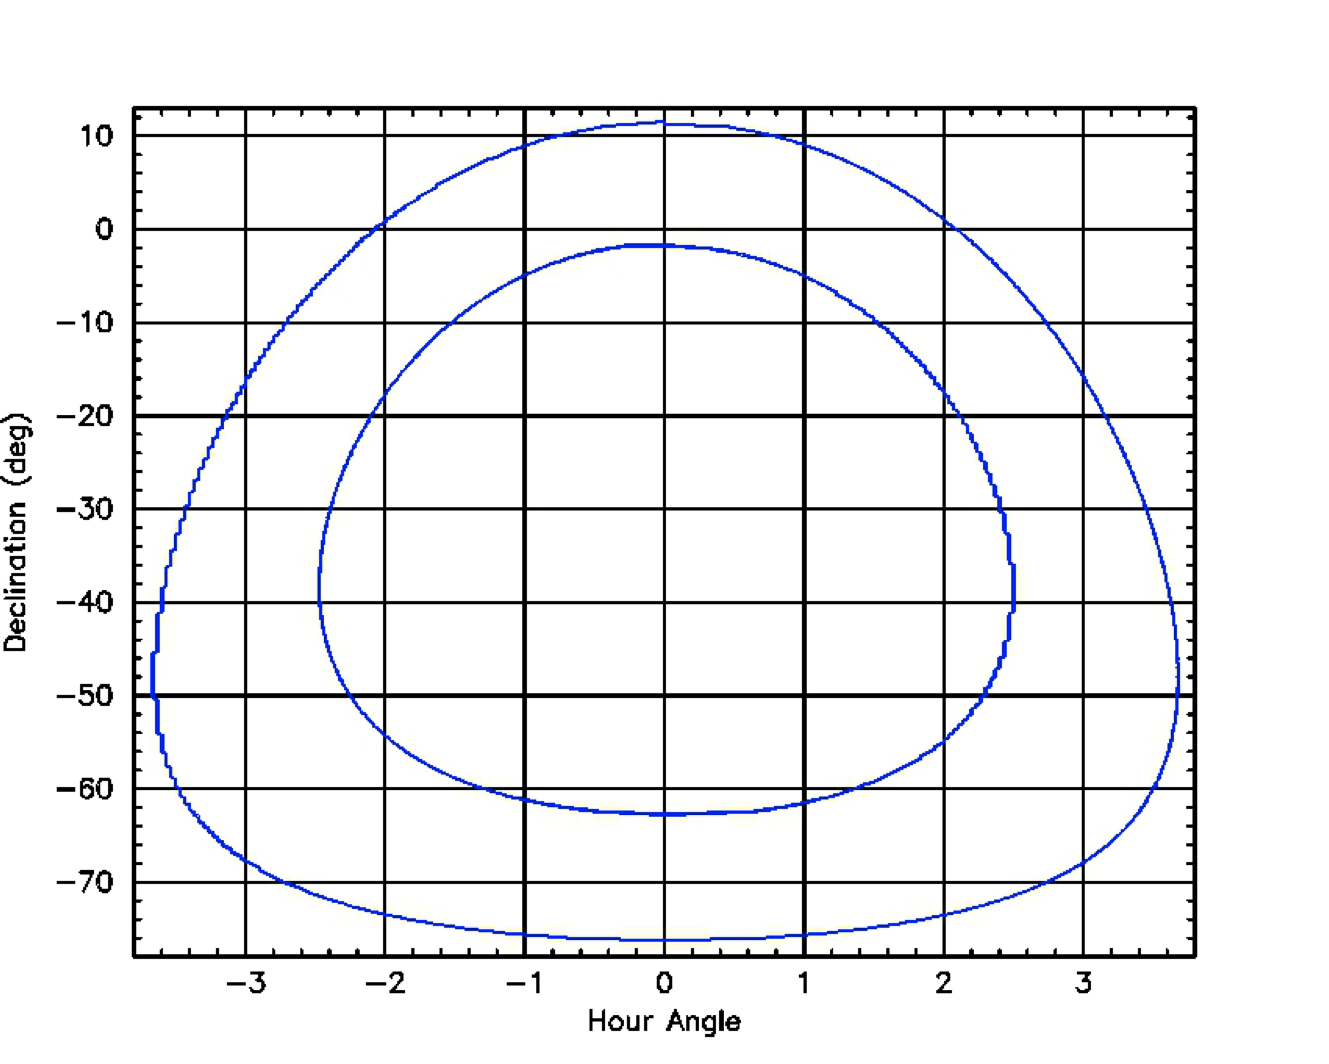
\includegraphics[width = 13cm]{figures/2_SALT_visibility.png}
    \caption{The visibility annulus of objects observable by SALT. Figure adapted from the SALT call for proposals (2013)\protect\footnotemark}
    \label{fig:SALT_visibility}
\end{figure}
\footnotetext{\protect\url{https://pysalt.salt.ac.za/proposal_calls/2013-2/}}

% Mention Center of Curvature Alignment System? : https://en.wikipedia.org/wiki/Shack%E2%80%93Hartmann_wavefront_sensor

The tracker is equipped with a 4 mirror spherical aberration corrector \citep{SALT_SAC}, and an atmospheric dispersion compensator \citep{SALT_ADC}, which corrects for the spherical aberration caused by the geometry of the primary mirror and allows access to wavelengths as short as 3200 \AA. These return a corrected flat focal plane with an 8\arcmin diameter field of view at prime focus on to the science instruments, with a 1\arcmin annulus around it used by the Tracker in a closed-loop guidance system.
\prgph

\subsection{The Robert Stobie Spectrograph}

SALT is equipped with the \gls{SALTICAM} and the \gls{RSS} science instruments onboard the tracker, and the \gls{HRS} and \gls{NIRifs} science instruments which are fibre-fed from the tracker to their own climate controlled rooms. The \gls{RSS} is the most used instrument on \gls{SALT} and the only instrument used for spectropolarimetry, and as such will be discussed in more depth than the other instruments.

The \gls{NIRifs} is currently being commissioned and will extend SALT's operational wavelength range from 3200 - 9000 \AA\ to 3200 - 17000 \AA, providing medium resolution spectroscopy at R = 2000 - 5000 over NIR wavelengths \citep{NIR, SALT_NIR}. This is ideally suited for studies of nearby galaxies.

The \gls{HRS} echelle spectrograph was designed for high resolution spectroscopy at R = 37000 - 67000 covering a wavelength range of 3700 - 8900 \AA\ and consists of a dichroic beam splitter and two \gls{VPH} gratings \citep{SALT_hires}. This instrument is capable of stellar atmospheric and radial velocity analysis.

The SALTICAM functions as the acquisition camera and simple science imager with various imaging modes, such as full-mode and slot-mode imaging, and supports low exposure times, down to 50 ms \citep{SALTICAM}. This enables photometry of faint objects, especially at fast exposure times.
\prgph

The \gls{RSS} functions as the primary spectrograph on \gls{SALT} and can operate in long-slit spectroscopy and spectropolarimetry modes, narrowband imaging mode, multi-object and high resolution spectroscopy modes, and low resolution Fabry-P\'erot imaging spectroscopy and tunable filter narrowband imaging modes \citep[for an in-depth discussion on operational modes see][]{SALT_operational_modes}.
\prgph

\todo{Optical layout (Figure) and description, and CCD/Lamps/Filters etc. available. Focus on spectropolarimetry and a short description on how observations are organized, gratings, spectral ranges, as well as the latest developments (PG0700, and anything else new)
    \prgph}

\section{RSS Spectropolarimetric Reductions} % In depth

\todo{How spectropolarimetry reductions differ from spectroscopy, polarimetry, and general spectropolarimetry reductions}

\subsection{General Reduction Process} % Rename?, In depth

\todo{
    \begin{itemize}
        \item How reductions would be done in general and through pure IRAF.
        \item I.E. Frames observed → flat, bias, arc, multiple targets, others(?)
        \item Corrections → flat fielding, bias subtraction (EQ from obs. astro), others(?)
        \item Calibrations → wavelength, flux, shifting (trace to center), background subtraction, others(?)
        \item Extraction → spectral extraction, others(?)
        \item \sout{Stokes parameter calculations / Post processing / Displaying / saving / comparing results}
    \end{itemize}
}

\subsection{POLSALT} % In depth

\todo{
    \begin{itemize}
        \item In depth but not a users guide, more focus on purpose than the parameters (I.E. why each step is necessary and draw comparison to general reduction)
        \item Why polsalt works without any major need for concern. "All steps except for the wavelength calibration and spectral extraction run with no user input. The spectral extraction is not a calibration but a simple check to make sure the entire trace is included in the window and also that the background regions do not contain any other objects lying on the frame or include the trace."
    \end{itemize}
}
\todo{
    Raw image reductions
    \begin{itemize}
        \item Bias/Dark/Flat/Fringe(?)/Crosstalk/Mosaicking
        \item All processes run / files created / PURPOSE!
    \end{itemize}
}
\todo{
    Wavelength calibrations
    \begin{itemize}
        \item Arc/Background subtraction/Cosmic ray rejection
        \item All processes run / files created / PURPOSE! / Heavy focus since supplementary pipeline replaces this step
    \end{itemize}
}
\todo{
    Spectral extraction
    \begin{itemize}
        \item All processes run / files created / PURPOSE!
        \item Raw Stokes calculations
        \item Wollaston ??
        \item All processes run / files created / PURPOSE!
    \end{itemize}
}
\todo{
    Final Stokes calculations
    \begin{itemize}
        \item All processes run / files created / PURPOSE!
    \end{itemize}
}
\todo{
    Post-processing analysis
    \begin{itemize}
        \item PURPOSE
        \item All 'script.py' steps in the BASH reduction
        \item Data Culling (BASH) (not used but mention use) /
        \item Flux Calibrations (BASH and errors in GUI (make 100\% sure about division error and notify Danielle before/if planning on including)) /
        \item saving plot and text pipeline results (BASH and GUI) /
        \item Synthetic Filtering (BASH) /
    \end{itemize}
    \begin{itemize}
        \item Mention bash script and GUI versions and differences, as well as what SALT's preferred method is
    \end{itemize}
}

\chapter{Developed Tools}

This chapter contains an overview of why supplementary tools were deemed necessary for an already working reduction process (\S~\ref{sec:polsalt_limits}), which aspects of the reduction process have been altered, replaced, or added (\S~\ref{sec:mod_tools}, \ref{sec:add_tools}), and finally what an updated reduction process consists of using a combination of all software (\S~\ref{sec:red_proc}).


\section{Limitations of POLSALT and the Need for a Supplementary Tool} \label{sec:polsalt_limits} % Rename

% Why
The creation of supplementary tools for \polsalt\ spectropolarimetric reductions stem from, primarily, the limitations of the wavelength calibration process and a need for a way to compare wavelength solutions across matching $O$ and $E$ polarization beams. Due to the time-consuming process of recalibrating the wavelength solutions it is not feasible to perform the wavelength calibrations time and time again for any amount of reductions larger than a handful of observations.
\prgph

% PG0300 reasoning
The prime motivation of finding an alternate method of wavelength calibrating the data stemmed from a large backlog of unused data taken using the $PG0300$. The only arc available for the $PG0300$ with a close enough articulation and grating angle ($\sim 10.68$ and $\sim 5.38$, respectively) was \gls{SALT}'s Argon lamp which displayed sparse spectral features with large gaps over the wavelength range at these grating and articulation angles. This often lead to inconsistent wavelength solutions, or failed altogether, through \polsalt, since minor deviations of identified spectral features may result in large deviations in regions with no spectral features.
\prgph

% How
The chosen solution was to use a well established tool to perform the wavelength calibration - one which allows for rapid recalibrations as well as provides a familiar interface with which the user can analyze their wavelength solutions. \iraf\ provides this familiar environment and reliability, even considering it's age and \hyperlink{https://github.com/iraf-community/iraf}{limited community development}. Unfortunately, \iraf\ is unable to natively parse the file structure implemented by \polsalt\ `as is' and formatting of the data structures are necessary for integration purposes. This restructuring works both ways as once the \iraf\ reductions are complete the format must be reformatted to match that of the \polsalt\ output such that the reduction process may carry on in \polsalt.
\prgph

\begin{figure}[t]
    \centering
    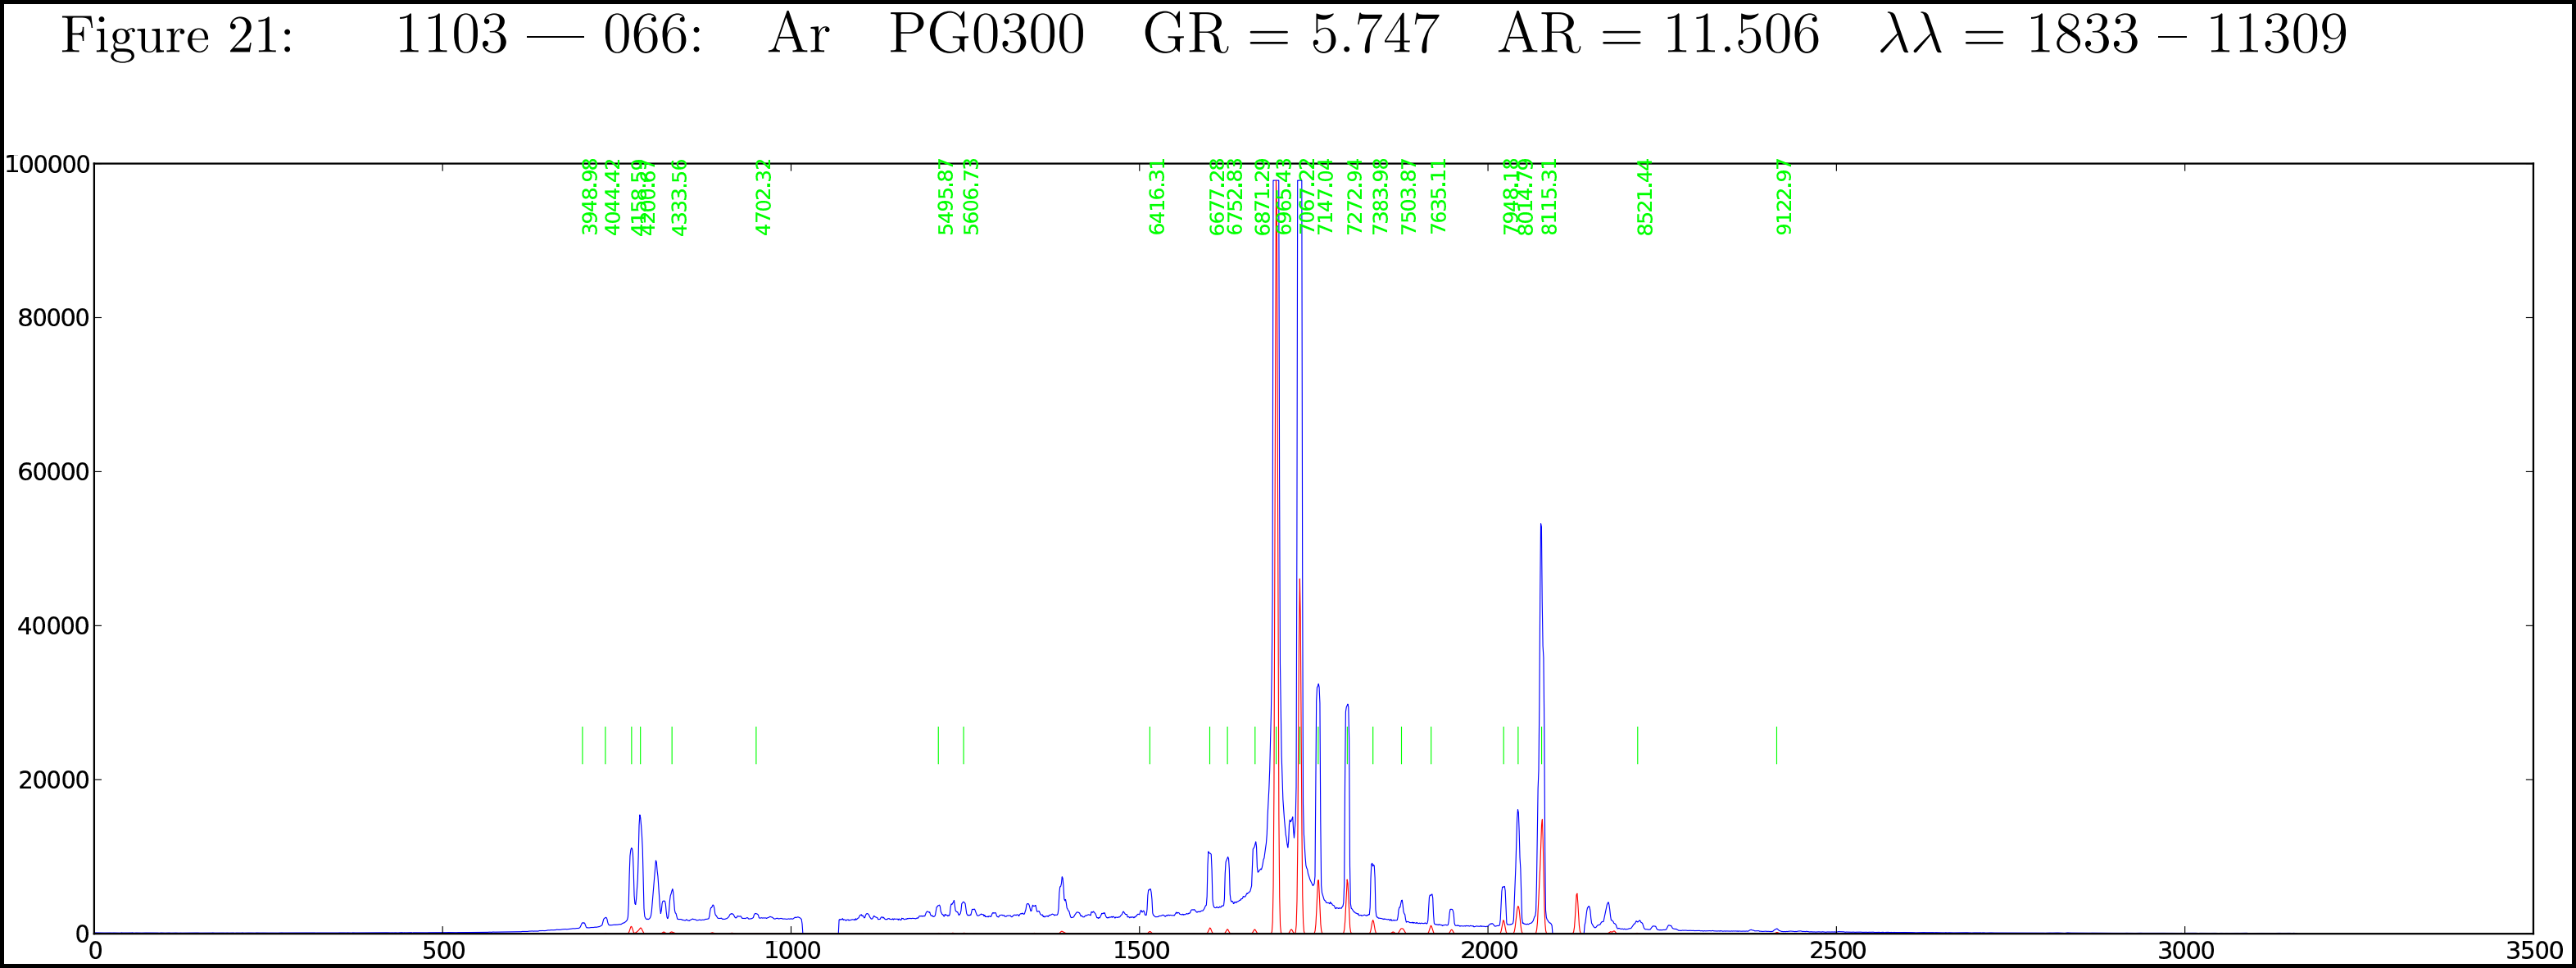
\includegraphics[width = 0.98\textwidth]{figures/3_arc_spectrum.png}
    \caption{One of many Argon arc lamp spectra as provided by \gls{SALT} for line identification. Plot adapted from \gls{SALT}'s published Longslit Line Atlases (as of 2024),\protect\footnotemark resized to fit within the document margins but otherwise unchanged.}
    \label{fig:ar_arc_salt}
\end{figure}
\footnotetext{\protect\href{https://pysalt.salt.ac.za/lineatlas/plot_line_argon_lores.pdf}{`low resolution' Ar plot} sourced from \protect\url{https://astronomers.salt.ac.za/data/salt-longslit-line-atlas/}}


\section{Wavelength calibrations - Supplementary Tools and IRAF} \label{sec:mod_tools}

The supplementary tools offer an alternate procedure for wavelength calibrations for the \polsalt\ pipeline. This procedure can be broken into three unique steps: the parsing of \polsalt\ data into an \iraf\ friendly format, referred to as splitting; the wavelength calibration performed in \iraf; and the reformatting of the data with its wavelength calibration back into the format expected by \polsalt, referred to as joining.

\begin{figure}[t]
    \centering
    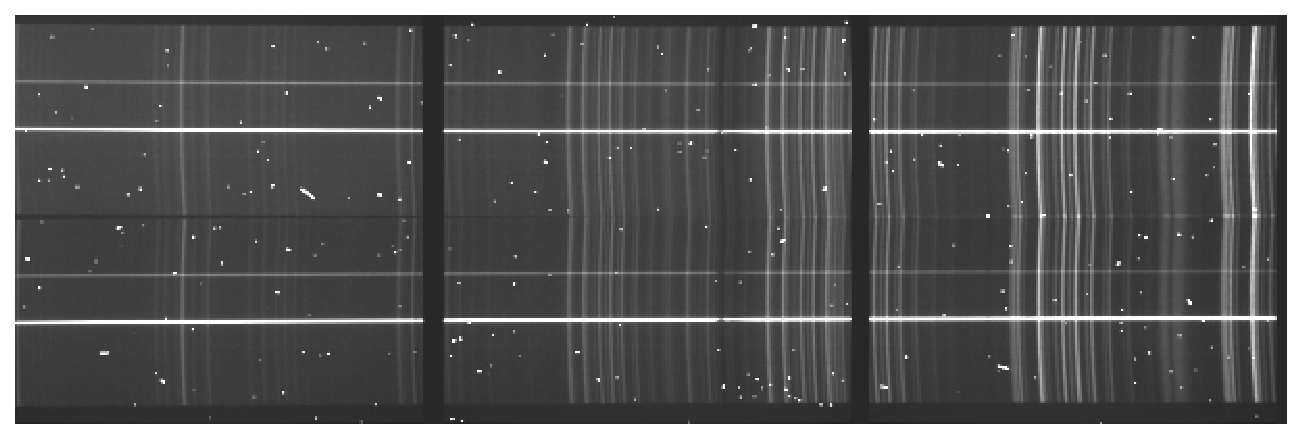
\includegraphics[width = 1.0\textwidth]{figures/3_pre_wav_cal.pdf}
    \caption{The science extension of a typical \polsalt\ \acs{FITS} file after basic \gls{CCD} reductions have been completed.}
    \label{fig:polsalt_pre_wav_cal}
\end{figure}


\subsection{Splitting the POLSALT pre-calibration files}

% Why necessary
%   Mention steps before and how they return (especially) the file structure.
As mentioned previously, the format of the \gls{FITS} file created by \polsalt\ after basic \gls{CCD} reductions and that expected by \iraf\ to be used for the wavelength calibrations are incompatible. A typical \gls{FITS} file created by the \polsalt\ basic \gls{CCD} reductions process contains a primary header along with the various image extensions, all of which include the trace for both polarimetry beams, as seen in Figure~\ref{fig:polsalt_pre_wav_cal}. \iraf\ deals best with a singular trace, and therefore a singular polarization beam, at a time.
\prgph

In an attempt to simplify the \iraf\ reduction procedure it was decided to split the polarization beams into their own files, as the parameters of \iraf\ tasks generally handle lists of files better than subregions of the same \gls{HDU}, and generally allowed for easier calibrations further down the \iraf\ wavelength calibration process.
\prgph

% What it does -> Primary focus
%   All processes run & description of each. Focus on why.
The \polsalt\ files with basic \gls{CCD} reductions applied, namely \gls{FITS} files with the prefix `mxgbp' (\S~\ref{subsec:polsalt}), are used as the starting point for the supplementary tool's \texttt{split} method. Running \texttt{split} finds all the \gls{FITS} files for wavelength calibration within the working directory, creates two empty \gls{HDU} structures for each sub-extension of the \gls{FITS} file, and appends all science and header data necessary for wavelength calibration to the relevant \gls{HDU} structure.
\prgph

% Focus on minimizing changes and optimizing size
As the intent was always to parse the wavelength function back into \polsalt\ it was decided to keep these temporary \gls{FITS} files as light as possible. This is especially necessary when considering the amount of frames that must be taken for a single spectropolarimetric observation, and then how the number of observations increases for long term studies.
\prgph

\begin{figure}[t]
    \centering
    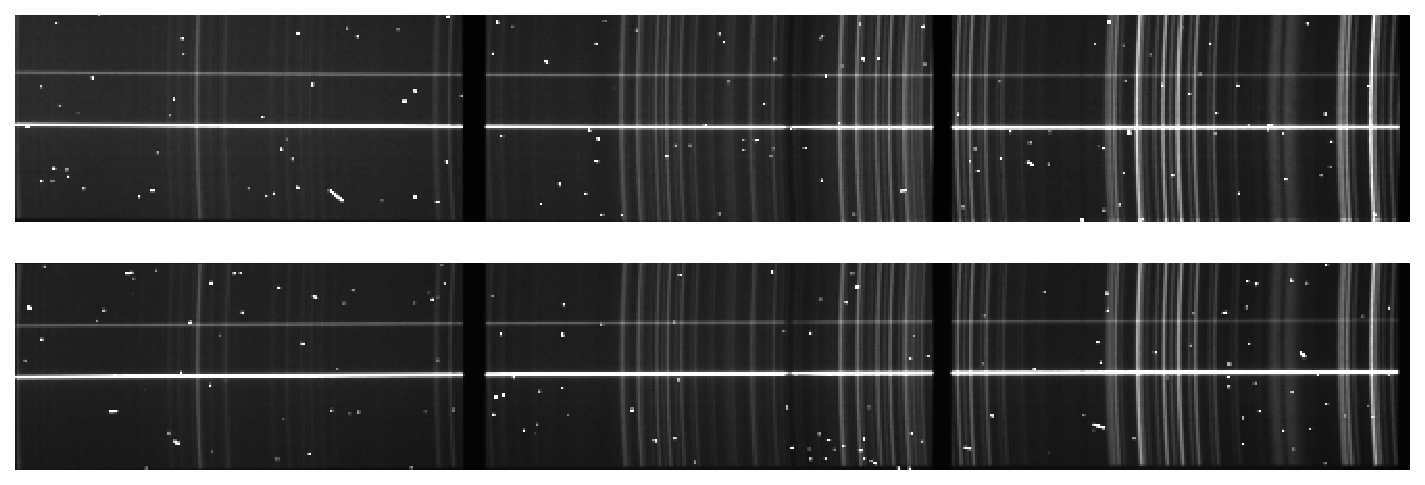
\includegraphics[width = 1.0\textwidth]{figures/3_OEsplit.pdf}
    \caption{The split $O$ and $E$ beams as handed to \iraf.}
    \label{fig:OE_split}
\end{figure}

% Any changes from how polsalt would do it
To aid the \iraf\ wavelength calibrations, row cropping and file list creation were introduced into the \texttt{split} method to ignore the regions without a trace either side of the frame, and to list the $O$ and $E$ beam \gls{FITS} files, respectively. The row cropping was decided on as \iraf\ does not handle the empty rows well, specifically when it comes to the \texttt{reidentify} task. Otherwise, defaults, such as which row to split the beams along, were kept as close to the \polsalt\ pipeline as possible.


\subsection{IRAF wavelength calibration}\label{subsec:IRAF_wav_cal}

% What is IRAF and why necessary
\iraf\ is a collection of software designed specifically for the reduction and analysis of astronomical images and spectra. The software consists of many tasks which perform specific operations and which are grouped into relevant packages. As every researcher, university, and research group have their own preferred wavelength calibration procedures and often use specific parameters for the various \iraf\ tasks (e.g. the order and type of the polynomial used in \texttt{identify}, etc.) only a brief overview of the tasks used will be provided here.
\prgph

A useful \iraf\ task that will not be discussed but nevertheless deserves a mention is the \texttt{mkscript} task in the \texttt{system} package which allows a user to create and save a task along with the defined parameters as a file which can later be called as a script. It is instrumental as a scripting aid and is what allows \iraf\ its rapid recalibrations of the wavelength solutions.
\prgph

For the alternate wavelength calibrations, the relevant tasks, in order, are \texttt{identify} and \texttt{reidentify} located in the \texttt{noao.onedspec} package, and the \texttt{fitcoords} and optionally the \texttt{transform} tasks located under the \texttt{noao.twodspec.longslit} package. These tasks produce a two-dimensional wavelength solution and thus must all be run twice to create the different wavelength solutions for each of the two spectropolarimetric beams.

% What it does -> Primary focus
%   All processes run & description of each. Focus on why.
% https://astro.uni-bonn.de/~sysstw/lfa_html/iraf/noao.onedspec.identify.html#h_29
% https://iraf.net/irafdocs/formats/identify.php
\paragraph{Identify}
The \texttt{identify} task is used to interactively determine a one-dimensional wavelength function across a chosen row of an arc exposure by identifying features in the spectrum with known wavelengths. \texttt{identify} gives the first approximation of the wavelength solution, which is saved to a local database, and is built on in subsequent tasks. It is thus imperative that the initial fit is done well to minimize errors further down the calibration process.
\prgph

The process of using \texttt{identify} consists of identifying known features spanning the entire wavelength range and then removing identified features which negatively impact the wavelength solution. A balance must be found between the number of identified features and parameters of the fit against the deviation of the fit from the known features. % RMS

% https://astro.uni-bonn.de/~sysstw/lfa_html/iraf/noao.onedspec.reidentify.html#h_29
\paragraph{Reidentify}
The \texttt{reidentify} task is used to run the \texttt{identify} task autonomously and repeatedly across the entirety of the arc exposure at a defined interval. \texttt{reidentify} uses the one-dimensional wavelength solution stored in the database created by the initial \texttt{identify} call and shifts the identified points to match their known spectral features. The task may fail based on a number of defined conditions, most common of which is the loss of features as the task moves further from the row at which the user ran \texttt{identify}.
\prgph

When running \texttt{reidentify} non-interactively, it is recommended to set the \texttt{verbose} parameter to `\texttt{yes}' as this will allow immediate confirmation whether the task quit early or not. Regardless of where the task ended, the newly defined wavelength solutions are appended to the local database.

% https://astro.uni-bonn.de/~sysstw/lfa_html/iraf/noao.twodspec.longslit.fitcoords.html
% https://iraf.net/irafdocs/formats/fitcoords.php
\paragraph{Fitcoords}
The \texttt{fitcoords} task is used to combine the collection of one-dimensional wavelength solutions in the local database to a two-dimensional surface function. This surface function is the final two-dimensional wavelength solution and is what is needed to convert the \iraf\ formatted wavelength calibrated \gls{FITS} files back into the \polsalt\ format.
\prgph

The process of using \texttt{fitcoords}, follows closely to that of \texttt{identify} and consists of examining the distribution of identified points and eliminating any points that \texttt{reidentify} may have misidentified. By eliminating outliers with bad residuals and modifying the two-dimensional surface function type and degree, the overall error of the fit decreases, matching more closely to what the `true' wavelength solution is.

% https://astro.uni-bonn.de/~sysstw/lfa_html/iraf/noao.twodspec.longslit.transform.html
\paragraph{Transform}
The \texttt{transform} task is an optional step in the \iraf\ wavelength calibration process but is good to perform since it is quick to run and easy to script. \texttt{transform} converts the ($pixel$, $pixel$) units stored in the exposure to ($wavelength$, $pixel$) units which allows for an immediate check of whether the wavelength solution was found correctly. Any error in the wavelength solution will be easily spotted in the transformed images and may range from minor, such as the arc exposure's arc lines or science exposure's sky lines not being straight across the columns of the frame, to more severe, such as the wavelength solution completely readjusting the frame to an incoherent mess.

\todo{Include poor and good transformed image examples?}


\subsection{Joining the wavelength calibrated files}

As mentioned previously, the format of the \gls{FITS} file created by \iraf\ after wavelength calibrations and that expected by \polsalt\ for the \texttt{spectra extraction} are incompatible. A typical \gls{FITS} file expected by the \polsalt\ \texttt{spectra extraction} contains a primary header along with the various image extensions, the most notable extension being the newly added wavelength extension. All images contained within the extensions have the trace for both polarimetry beams split, as seen in Figure~\ref{fig:polsalt_post_wav_cal} and the headers of each extension updated.
\prgph

All pieces necessary to recreate the \polsalt\ wavelength calibrated \gls{FITS} files exist once the \iraf\ procedure to generate the database entry for the two-dimensional wavelength solution is complete. The \texttt{join} method of the supplementary tools is used at this point and, once run, automatically creates the desired files.
\prgph

Running \texttt{join} finds all the relevant \gls{FITS} and local database files necessary to run the \polsalt\ \texttt{spectra extraction}, creates an empty \gls{HDU} structure for each pair of matching spectropolarimetric beams, copies over the extensions and their respective image and header information, checks and corrects the trace splitting to best match that of \polsalt, appends a new extension and parses the database wavelength solutions into the \polsalt\ intensity-wavelength format, cleans the science extension for cosmic rays, and does some house-cleaning to align the finalized \gls{FITS} files to those created when using the `pure' \polsalt\ pipeline.
\prgph

% update headers
% copy data, double check shape change
The \gls{FITS} files created by the \texttt{join} method and \polsalt\ pipeline's \texttt{wavelength calibration} methods are almost identical. The only difference between the \gls{FITS} files is the shape of the images stored within them, reflected also through specifically the `NAXIS2' header keyword, since \texttt{split} introduces a cropping. It was deemed unnecessary to reintroduce the cropped region as it is promptly discarded in the following \polsalt\ \texttt{spectra extraction} process and raises no issues when left out. Otherwise, both the \texttt{join} method and \polsalt\ \texttt{wavelength calibration} update the headers to reflect the new shape of the data and data type, through header keywords `CTYPE3' and `BITPIX', respectively.
\prgph

% append new extensions
% How db converted to wav func
% parse and save wavelength functions as image
The wavelength extension is created entirely by \texttt{join} by appending a blank extension to the \gls{HDU} and filling the image pixels with their respective wavelength value. This is done entirely by \texttt{join} which parses the wavelength database file and creates a function which provides the corresponding wavelength when provided with a ($pixel$, $pixel$) position. This is used to fill the pixels of the wavelength extension with their respective wavelength, as seen in Figure~\ref{fig:pol_wav_ext}. Note that regions that fall outside the trace are masked by setting the wavelength extensions corresponding pixel value to $0$.
\prgph

\begin{figure}[t]
    \centering
    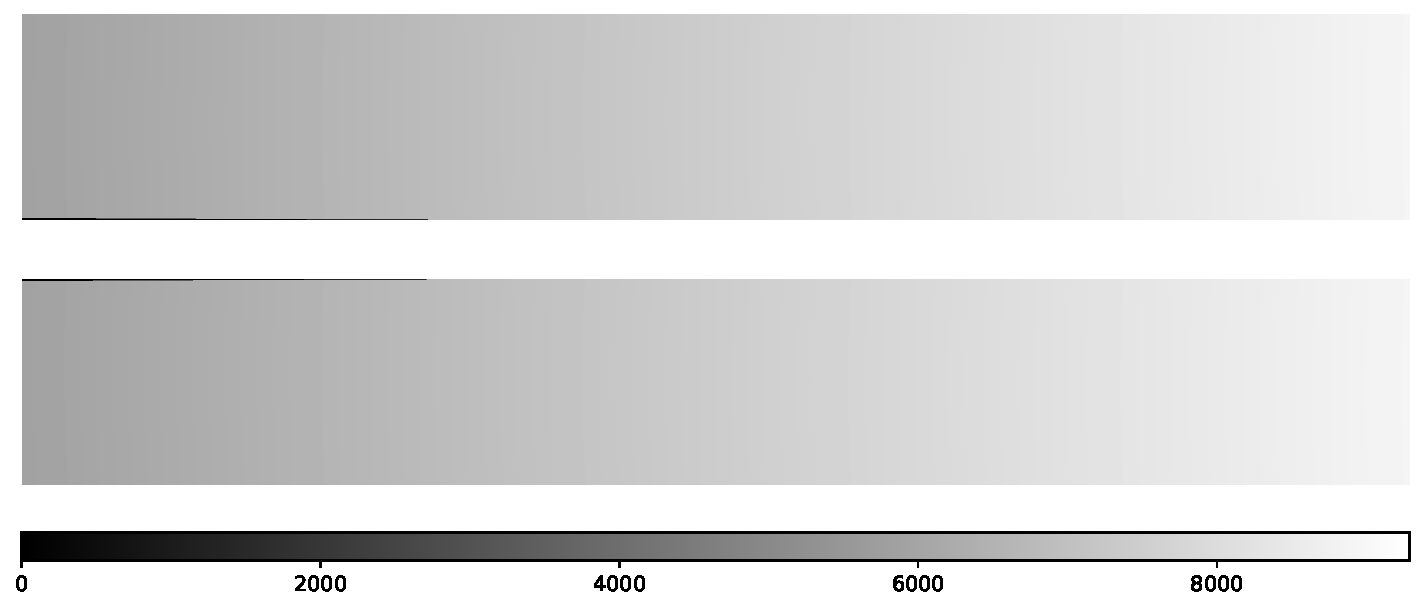
\includegraphics[width = 1.0\textwidth]{figures/3_pol_wav_ext.pdf}
    \caption{The wavelength extension of a \gls{FITS} file ready to be handed back to the \polsalt\ pipeline.}
    \label{fig:pol_wav_ext}
\end{figure}

% cosmic ray cleaning
\texttt{join} cleans the science extension of cosmic rays using the \texttt{lacosmic} python package which was specifically designed for this purpose and uses the L.A. Cosmic algorithm, based on Laplacian edge detection. The parameters used for cosmic ray cleaning were chosen based on the properties of the \gls{RSS}, specifically the read noise and gain, as well as a publication and \hyperlink{http://www.astro.yale.edu/dokkum/lacosmic/pars.html}{suggestions} by the algorithm's creator \citep{lacosmic}. The chosen parameters work well for all but the worst of cosmic rays, as can be seen when comparing Figures~\ref{fig:OE_split} and \ref{fig:polsalt_post_wav_cal}.
\prgph

% polsalt specific cropping (wav mask)
% mask wavelength using wollaston curve for polsalt `parsability'
% update BPM to reflect wavelength cropping
The wavelength extension is masked to remove any impossible wavelengths and also corrected for the skewing of the trace introduced by the wollaston element. The skewing must be added to the wavelength extension since \polsalt\ introduces a wollaston correction in the \texttt{spectra extraction} process. Finally, the \gls{BPM} extension is masked to reflect the valid wavelength calibrated regions for both spectropolarimetric beams and the files are saved with the \polsalt\ wavelength calibrated `wmxgbp' prefix.

\begin{figure}[t]
    \centering
    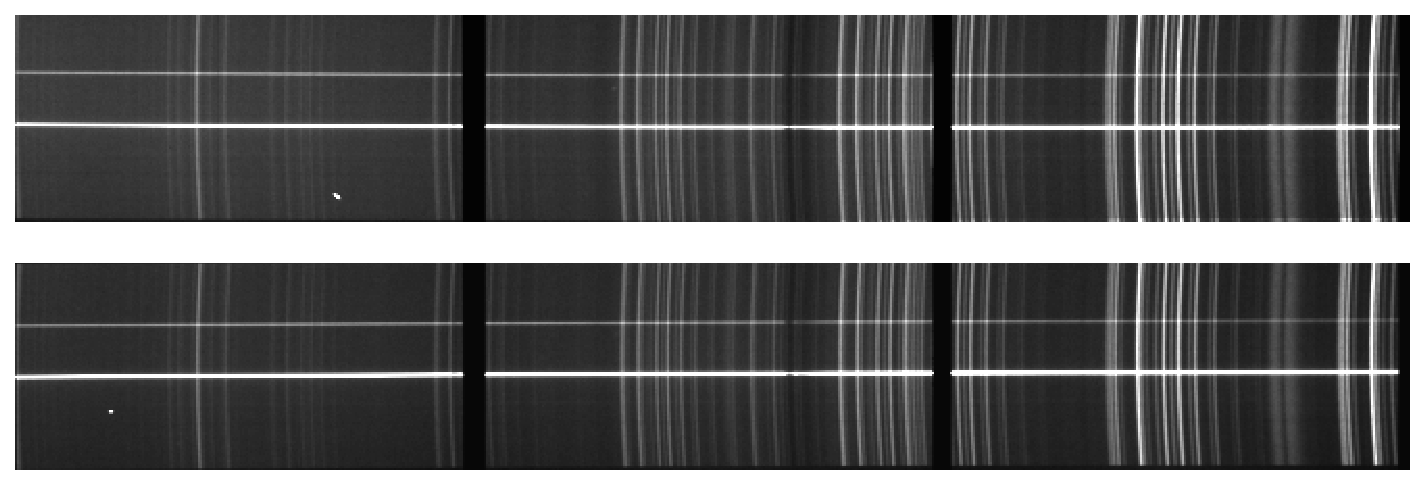
\includegraphics[width = 1.0\textwidth]{figures/3_post_wav_cal.pdf}
    \caption{The science extension of a \gls{FITS} file ready to be handed back to the \polsalt\ pipeline.}
    \label{fig:polsalt_post_wav_cal}
\end{figure}


\section{Additional Tools}\label{sec:add_tools}

Before creating the supplementary tool's \texttt{split} and \texttt{join} methods used to perform wavelength calibrations in \iraf, it was deemed necessary to create tools to allow for the comparison of the $O$ and $E$ beams wavelength solutions.


\subsection{Sky line comparisons}

Sky line comparisons serve two unique yet interconnected services. Firstly, they naively transform the wavelength calibrated frame, without conserving flux, allowing the user confirmation of the variation of sky lines across the columns of the frame, and secondly, they compare the wavelength position of the sky lines with the \gls{SALT} sky lines,\footnote{The first iteration of a sky line atlas is available at \url{https://astronomers.salt.ac.za/data/salt-longslit-line-atlas/}} allowing confirmation of the wavelength solution at positions across the rows of the frame. The file used for skyline comparisons may be the \iraf\ \texttt{transform} \gls{FITS} file, which allows for flux conservation through the `\texttt{flux}' parameter.
\prgph

The \texttt{skyline} method loads the wavelength calibrated files, transforms the frames (as described above) if the frame was not transformed by \iraf's \texttt{transform} method, divides out the continua, compares the averaged cross-column sky lines to those of a single row, and compares the wavelength position of said sky lines to those known by \gls{SALT}.


\todo{Give more detail when properly implemented in code. Discuss arguments (both compulsory and optional)}


\subsection{Cross correlation}

Cross correlation allows for the comparison of the features in signals. This is useful when dealing with spectropolarimetric spectra as it allows a comparison of how well aligned the spectra are wavelength-wise. Using this, we can determine if any misidentifications had skewed the entire wavelength solution, as compared to the \texttt{skyline} method which allows identification of singular misidentifications within the wavelength solution.
\prgph



\todo{
    \begin{itemize}
        \item Why cross correlation
        \item discussion of script processes (how it works)
        \item discuss all arguments provided to method
    \end{itemize}
}


\section{General Reduction Procedure}\label{sec:red_proc}

\begin{figure}[t]
    \centering
    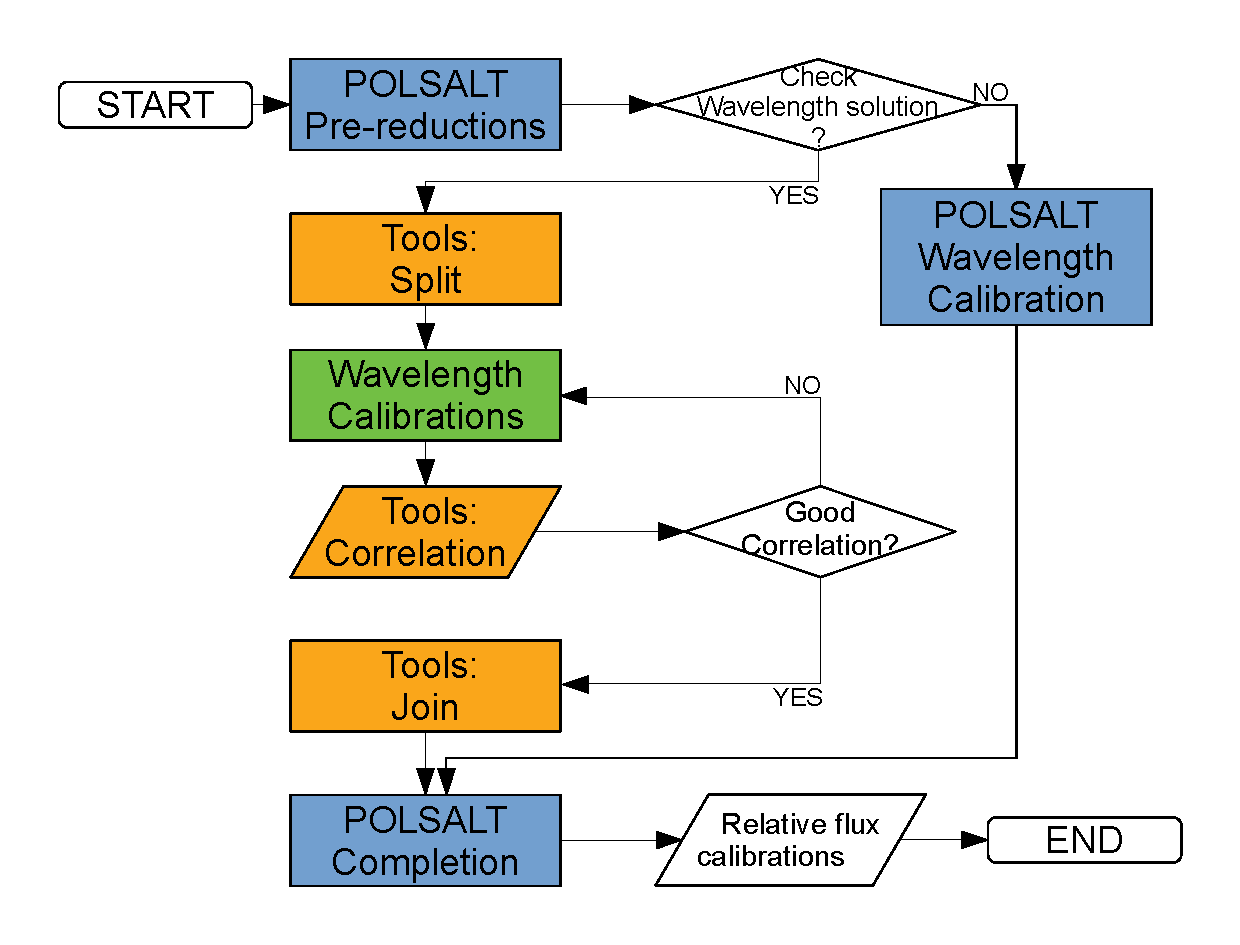
\includegraphics[width = 0.8\textwidth]{figures/3_new_workflow.pdf}
    \caption{A general workflow for data reductions using a combination of \polsalt, \iraf, and the developed supplementary tools.}
    \label{fig:new_workflow}
\end{figure}

This section aims to give an overview of the reduction procedure from start to finish and to cover all commands needed to achieve a finalized result. As users all employ a variety of operating systems, language environments, and software setups, not much emphasis will be placed on how to get the software running or the managing of files, only the commands necessary to complete each step of the reduction process, assuming that the software is running as intended.
\prgph

It is recommended that \polsalt\ is used through the \gls{GUI} as it provides a user-friendly environment while also sequentially listing each step of the reduction process in a dropdown menu. Reductions are possible, however, purely using a \gls{CLI} and the \polsalt\ scripts. It is assumed that usage of \polsalt\ through the \gls{GUI} or \gls{CLI} use the `beta' or `basic' versions, respectively, and that both versions are run from the \polsalt\ directory. The \iraf\ terminal, once launched, and the \gls{CLI} supplementary tools are assumed to be run from the `working' directory. This ensures that commands containing \texttt{<.../>} notate relative paths to the desired file or folder.
\prgph

Help documentation, primarily describing the possible arguments, is available in the \gls{CLI} for \polsalt\ and the supplementary tools using the \texttt{-h|--help} flag with their respective invocation, such as:

\begin{verbatim}> python <.../>Masters split --help\end{verbatim}

\noindent and for \iraf\ through the \texttt{?|:.help} `cursor mode' options while running an interactive task.


\subsection{POLSALT Pre-reductions}\label{subsec:reduc_pre}

\polsalt\ requires a file structure such that the raw data received from \gls{SALT} is located in a folder labeled using the observing date as well as being in a sub-folder labeled raw, such as \texttt{YYYYMMDD/raw/}. This directory structure allows \polsalt\ to create a `working' directory named \texttt{YYYYMMDD/sci/} which contains all the files modified during the reduction process. This allows for separation of reductions of the same data by simply renaming the \texttt{sci/} directory.
\prgph

To launch the \gls{GUI}, navigate to the \polsalt\ directory within a \gls{CLI} and run:

\begin{verbatim}> python -W ignore reducepoldataGUI.py &\end{verbatim}

\noindent Once the window has launched, ensure that the first and second paths at the top of the window point to the \polsalt\ and data observation date directories, respectively. The `raw image reduction' may then be selected from the dropdown and run. The \polsalt\ \gls{CLI} command:

\begin{verbatim}> python scripts/reducepoldata.py <.../>YYYYMMDD\end{verbatim}

\noindent then runs the raw image reduction process. It should be noted that the \polsalt\ \gls{CLI} command will, by default, attempt to run the wavelength calibration process. This behavior may be stopped by using the \texttt{-w} flag when running the command.
\prgph

\todo{Include screenshot of GUI, reference in paragraph above}


\subsection{Wavelength Calibration} \label{subsec:reduc_wav}
\todo{Create subsubsections for split, iraf, join, and the optional tools (including transform)?}

Splitting the data in the working \texttt{sci/} directory may then be done using:

\begin{verbatim}> python <.../>Masters split\end{verbatim}

Multiple default parameters are used, the most notable of which are the directory, which defaults to the current working directory of the \gls{CLI}, the split row, which defaults to \polsalt's default center row, and the save prefix, which defaults to `\texttt{obeam}' and `\texttt{ebeam}'. As an aside, the save prefix may be worth changing as, later in the reduction process, the \polsalt\ raw stokes reductions indiscriminately selects files named \texttt{YYYYMMDD/sci/e*.fits}.
\prgph

Moving on to \iraf, the wavelength calibrations are performed using the tasks described in \S~\ref{subsec:IRAF_wav_cal}, namely \texttt{identify}, \texttt{reidentify}, and \texttt{fitcoords}, and may be run directly in the \iraf\ terminal using:\footnote{Please see the \iraf\ help docs, available at \url{https://astro.uni-bonn.de/~sysstw/lfa_html/iraf/iraf.html}, on the relevant tasks for a comprehensive discussion of the parameters available.}

\begin{verbatim}
cl> identify images
cl> reidentify reference images
cl> fitcoords images fitname
\end{verbatim}

\noindent where `images' refer to a list or file containing the \gls{FITS} files relevant to the task, `reference' refers to the \gls{FITS} file previously identified, and `fitname' refers to the name to be used for the final two-dimensional wavelength solution. The interactive tasks take up the bulk of the reduction time as this is where the fine-tuning of the reduction is done, through the use of cursor commands (otherwise known as colon commands), which allow modification of the parameters mid-reduction. Task parameters may, however, be edited beforehand within the \iraf\ terminal using the \texttt{eparam} task, and optionally saved, and quit or run using a combination of \texttt{:w}, and \texttt{:q} or \texttt{:go} cursor commands, respectively.
\prgph

It is recommended to create an \iraf\ Command Language (cl) script for each task to keep track of which parameters were used and for simple recalibrations. The scripts are created using:

\begin{verbatim}cl> mkscript script_name.cl\end{verbatim}

\noindent which will interactively ask for the task and parameters to be used. Multiple tasks may be appended to an \iraf\ script, allowing for the parameters of both beams to be tracked. Running an \iraf\ script may be done by running:

\begin{verbatim}cl> cl < script_name.cl\end{verbatim}

\noindent but is not suggested for interactive scripts, which run best when simply copied from the \texttt{<.../>sci/script\_name.cl} file to the \iraf\ terminal.
\prgph

Joining the separate beams with their respective wavelength solutions may now be completed using:

\begin{verbatim}> python <.../>Masters join\end{verbatim}

Similar to the \texttt{split} procedure mentioned before, the \texttt{join} procedure has the same defaults defined and so a user must keep track of which defaults were changed and keep them consistent between the two tasks.
\prgph

\todo{
    \begin{itemize}
        \item Running cross correlation - discussed here but only truly done after spectra extraction, check variation between beams.
        \item Running skyline checks - skyline `can' use transformed images, check variation across the frame (both axes)
    \end{itemize}
}
\prgph

Finally, at least for reductions using \iraf, the optional \texttt{transform} task may be run using:

\begin{verbatim}cl> transform images output fitnames\end{verbatim}

\noindent where `images' refers to the same pseudonym as used in the previous \iraf\ task usage examples, `output' refers to the new file name for the transformed input images, and `fitnames' refers to the two-dimensional wavelength function name created by the \texttt{fitcoords} task.


\subsection{POLSALT Reduction Completion} \label{subsec:reduc_com}

Reductions may now be completed using \polsalt.

\todo{
    \begin{itemize}
        \item Deletion of o and e beam fits (due to POLSALT naming conventions and to save memory)
        \item POLSALT completion up to and including plotting
        \item relative flux calibrations for spectrum shape corrections if a standard observation available
    \end{itemize}
}
% % MARK: Testing
% \chapter{Testing}

% This chapter contains an overview of the testing performed for and during the development of \stops. The tests are divided into two main categories: \stops\ software tests (\autoref{sec:test_stops}) and reduction specific tests (\autoref{sec:test_reduction}). Software tests cover the methods implemented and error handling in \stops, specifically for \texttt{split} (\autoref{subsec:test_split}), \texttt{join} (\autoref{subsec:test_join}), \texttt{correlate} and \texttt{skylines} (\autoref{subsec:test_corr_sky}), while reduction tests cover verifying the alternate wavelength solutions (\autoref{subsec:test_wavelength}) and polarization parameters (\autoref{subsec:test_polarization}).

% % MARK: Software tests
% \section{\stops\ Development} \label{sec:test_stops}

% As development is an iterative process, only the major tests that were performed are discussed. The tests were, predominantly, to ensure that the input to \stops\ is parsed correctly and that the output of the relevant \stops\ methods align with the expected input for the relevant \iraf\ or \polsalt\ tasks.

% % Which tools were used/replaced/improved
% The key improvements and replacements made during the development of \stops\ included optimizing the file parsing process to streamline the swapping between the required \polsalt\ and \iraf\ file structures. Additionally, legacy functions used in \polsalt\ which were re-implemented in \stops\ were updated to Python 3 to ensure compatibility with the latest Python versions.

% % Why the pipeline is better
% The rigorous error handling in \stops\ ensures that the user is informed of any issues that arise during the reduction process. This is particularly important as \stops\ was developed to enable a faster reduction process compared to that of pure \iraf\ or \polsalt.

% % MARK: Split tests
% \subsection{Testing the \stops\ \texttt{split} method} \label{subsec:test_split}

% The \texttt{split} method was tested to ensure that the data output matched the expected format for \iraf. These tests included:
% \begin{itemize}
%     \item Verification of file structure and data integrity post-split.
%     \item Comparison of key data parameters between \stops\ and \iraf\ outputs.
%     \item Testing with various data sets to ensure robustness.
% \end{itemize}

% \todo{Insert table comparing key output parameters of \stops\ and \iraf\ split method.}

% \todo{Insert figure showing example output files from both methods.}

% % MARK: Join tests
% \subsection{Testing the \stops\ \texttt{join} method} \label{subsec:test_join}

% The \texttt{join} method in \stops\ was tested to ensure compatibility and correctness of the output data in comparison to \polsalt. This involved:
% \begin{itemize}
%     \item Matching the joined output with \polsalt\ outputs.
%     \item Ensuring the Wollaston correction was accurately applied.
%     \item Testing the integration of Python 3 updates.
% \end{itemize}

% \todo{Insert figure showing comparison of spectra before and after join operation.}

% \todo{Insert table summarizing differences in outputs (if any) between \stops\ and \polsalt.}


% % MARK: Cross Correlate/Skylines tests
% \subsection{Testing the \stops\ \texttt{correlate} and \texttt{skylines} methods} \label{subsec:test_corr_sky}

% The \texttt{correlate} and \texttt{skylines} methods were tested for accuracy and performance. Key aspects of the testing included:
% \begin{itemize}
%     \item Verifying the accuracy of the cross-correlation function against known standards.
%     \item Ensuring skyline identification was accurate and consistent.
%     \item Performance testing with large data sets to ensure efficiency.
% \end{itemize}

% \todo{Insert graph showing correlation results with known standards.}

% \todo{Insert figure illustrating skyline identification accuracy.}

% % MARK: Reduction tests
% \section{Reduction specific tests} \label{sec:test_reduction}

% Reduction specific tests refer to tests performed to ensure no errant effects are introduced during the reduction process. These tests were designed to validate the accuracy and reliability of the \stops\ pipeline in producing scientifically accurate results.

% % General discussion of sources used as part of testing
% The sources used for testing included a range of spectropolarimetric standards, both highly polarized and non-polarized objects. The tests aimed to check for issues such as data integrity, consistency of wavelength calibration, and accuracy of polarization measurements.

% \todo{
%     \begin{itemize}
%         \item General discussion of testing (I.E. not this test was done specifically this source, more along the lines of these tests were done to check this issue, seen here using this source for example.)
%     \end{itemize}
% }

% % MARK: Wavelength tests
% \subsection{Wavelength Solutions} \label{subsec:test_wavelength}

% Wavelength solution tests were conducted to validate the accuracy of the \stops\ wavelength calibration process. This included:
% \begin{itemize}
%     \item Full frame wavelength solution checks to ensure comprehensive calibration.
%     \item O/E correlation checks to verify the consistency of the wavelength solutions.
%     \item RMS comparisons between \polsalt\ and \stops\ to quantify differences.
% \end{itemize}

% \todo{Insert table comparing RMS values of wavelength solutions from \polsalt\ and \stops.}

% \todo{Insert figure showing full frame wavelength solution plots.}

% % MARK: Polarization tests
% \subsection{Polarization Parameters} \label{subsec:test_polarization}

% The accuracy of polarization parameters was tested using several known sources, including:
% \begin{itemize}
%     \item 3C 279
%     \item 4C+01.02
%     \item Data provided by David (preliminary testing data, not included in publications but used during pipeline development)
% \end{itemize}

% % MARK: Spectropolarimetric Standards
% \subsubsection{Spectropolarimetric Standards}

% Testing included the use of spectropolarimetric standards, comprising four highly polarized and two non-polarized objects. The specific tests performed were:
% \begin{itemize}
%     \item Background information on each object.
%     \item Detailed reductions steps performed on each object.
%     \item Comparison of \polsalt\ results to those obtained using the \stops\ pipeline.
% \end{itemize}

% \todo{Insert table listing the spectropolarimetric standards used, with their properties.}

% \todo{Insert figure showing comparison plots of polarization parameters from \polsalt\ and \stops.}

\chapter{Testing and Application}

Short intro to chapter contents.

\begin{itemize}
    \item No \polsalt\ or data tests
    \begin{itemize}
        \item \polsalt\ is trusted to be accurate. See \dots (reference tests of \polsalt)
    \end{itemize}
    
    \item Testing \texttt{split}
    \begin{itemize}
        \item \polsalt\ to \iraf\ file structure conversion.
        \item Show changes to data files are intended (I.E. only splitting the data, no changes to the data itself)
        \item Tested over multiple grating/articulation angles to ensure robustness.
        \item Mention any header updates skipped specific to \polsalt\ (if any)
        \item Figure showing split fits file contents difference (cropped rows shown, etc.)
    \end{itemize}
    
    \item Testing \iraf\ wavelength solution
    \begin{itemize}
        \item \iraf\ is trusted to be accurate. See \dots (reference tests of \iraf)
        \item The \texttt{skylines} and \texttt{correlate} outputs are tests of the wavelength calibration.
        \begin{itemize}
            \item Testing correlate functionality using `offset', comparisons of arcs, FSRQ's and BLLac's.
            \item Any figures showing correlation tests?
            \item Testing skylines using known spectral sky lines.
            \item Any figures showing skyline tests?
        \end{itemize}
    \end{itemize}

    \item Testing \texttt{join}
    \begin{itemize}
        \item \iraf\ to \polsalt\ file structure conversion
        \item Show changes to data files are intended (I.E. only joining the data, and `WAV' appended. No changes to the data itself)
        \item Wollaston correction of wavelength and bpm extensions
        \item update to python 3 of `polsalt' functions
        \item Mention any header differences (if any)
        \item Figure showing joined fits file contents difference (cropped rows shown once again, bpm differences due to CRR and NO wollaston bpm differences, etc.)
    \end{itemize}

    \item Testing reduction results not negatively impacted by \stops.
    \begin{itemize}
        \item General discussion of testing (I.E. not this test was done specifically this source, more along the lines of these tests were done to check this issue, seen here using this source for example.)
        \item Wavelength solution validation from correlate and skylines results.
        \begin{itemize}
            \item Figures showing Correlate and Skyline results.
            \item RMS comparisons between \polsalt\ and \iraf\ to quantify differences.
            \item Any Figures for RMS comparisons or wavelength validation?
        \end{itemize}
        \item Polarization parameters validation from known sources.
        \begin{itemize}
            \item Polarization tested using 3C 279, 4C+01.02, and preliminary testing data provided by David.
            \item Polarization tested using spectropolarimetric standards (4 highly polarized, 2 non-polarized).
            \item Tabulate sources used, with their properties.
            \item Figures showing comparison plots of polarization parameters from \polsalt\ and \stops.
        \end{itemize}
    \end{itemize}
\end{itemize}

\begin{itemize}
    \item Background information on each object.
    \item Detailed reductions steps performed on each object.
    \item Comparison of \polsalt\ results to those obtained using the \stops\ pipeline.
\end{itemize}

\begin{itemize}
    \item Application to Spectropolarimetric Standards
    \begin{itemize}
        \item Science results, what the results can tell us and why it is useful, also comparison of results to FORS1/2 published data, focus on the polarization results.
    \end{itemize}
    
    \item Application in Publications
    \begin{itemize}
        \item Summarize the results of the publications appended to appendix.
    \end{itemize}
\end{itemize}
\chapter{Science Applications}

\todo{Short introduction to chapter contents}

\section{Application to Spectropolarimetric Standards}
\todo{Spectropolarimetric standards (4 highly polarized, 2 non-polarized)
    \begin{itemize}
        \item (Same as ch04 with science results)
        \item Background on objects
        \item Reductions
        \item Actual results - comparison of polsalt results to supplementary pipeline results
        \item Science results, what the results can tell us and why it is useful, also comparison of results to FORS1/2 published data, focus on the polarization results
    \end{itemize}
}

\section{Application in Publications}

\todo{Summary of results from papers in appendix.
    \begin{itemize}
        \item Hester paper(s)
        \item Joleen proceedings and work
        \item My proceedings
    \end{itemize}
}

\todo{3C 279 and 4C+01.02
    \begin{itemize}
        \item Give Background on objects, Reduction steps, and Science results (what the results can tell us and why it is useful)
        \item (comparison of polsalt results to supplementary pipeline results will be in testing)
    \end{itemize}
}

\chapter{Conclusions}

\todo{A summary of the dissertation, main focus on the results and that the supplementary pipeline is a success since it allows an alternate method using IRAF to wavelength calibrate the polsalt data.}

% MARK: Acknowledgements
\begin{acknowledgements}
    I hereby acknowledge and express my sincere gratitude to the following parties for their valuable contributions:
    \begin{itemize}
        \item \todo{Add acknowledgements!}
            % \item Brian van Soelen, for his support as supervisor.
            % \item My family, both near and far, for all the encouragement and support that they offered.
            % \item The team at SALT, specifically David Buckley and Danièl Groenewald for their time and expertise.
            %   All/some [choose which is appropriate] of the observations reported in this paper were obtained with the Southern African Large Telescope (SALT) under program(s) [insert Proposal Code(s)].
    \end{itemize}
\end{acknowledgements}
\printglossary[type=acronym, title={List of Acronyms}] %[type=abbreviations, style=alttree, title={List of Acronyms}]


\bibliographystyle{plainnat} %{aasjournal} (surnames first) %{humannat}
\bibliography{references}

% \begin{appendices}
% \input{Chapters/AppendixPub}
% \end{appendices}

\end{document}
